\documentclass[12pt,a4paper]{book}
\usepackage[utf8]{inputenc}
\usepackage[english]{babel}
\usepackage[left=2cm,right=2cm,top=2cm,bottom=2cm]{geometry}

\usepackage{amsmath}
\usepackage{amsfonts}
\usepackage{amssymb}

\usepackage{graphicx}				% import external graphics ( \includegraphics command)
\usepackage{wrapfig}					% allow text to wrap around figures ( \begin{wrapfigure} )
\usepackage{subcaption}			% allows subfigures within figures. Subfloats have their own caption, and an optional global caption.

\usepackage{siunitx}					% standard international system of units of measurement

\usepackage{varioref}				% verbose references package
\usepackage{hyperref}				% references and links package
\hypersetup{
%    bookmarks = true,         	% show bookmarks bar?
    unicode = false,          	% non-Latin characters in Acrobat’s bookmarks
    pdftoolbar = true,        	% show Acrobat’s toolbar?
    pdfmenubar = true,        	% show Acrobat’s menu?
    pdffitwindow = false,     	% window fit to page when opened
    pdfstartview = {FitH},    	% fits the width of the page to the window
    pdftitle   =								% title
    		{Photonic Artificial Neural Networks},
    pdfsubject = 							% subject of the document
    		{Application of integrated silicon photonics to artificial neural network design},
    pdfauthor  = {Davide Bazzanella},		% author
    pdfcreator = {Davide Bazzanella},  	% creator of the document
    pdfkeywords={integrated, photonic,		% list of keywords
    							microring, resonator,		%
    							neural, network,					%
    							feedforward}, 						%
    pdfnewwindow = true,	% links in new PDF window
    colorlinks = true,		% false: boxed links; true: colored links
    linkcolor = black,		% color of internal links (change box color with linkbordercolor)
    citecolor = black,		% color of links to bibliography
    filecolor = black,		% color of file links
    urlcolor  = blue			% color of external links
}
\usepackage{cleveref}				% clever references package

\usepackage{caption}			% Nice captions
\captionsetup{
		format			= hang,		% Indents the caption text, so it will ‘hang’ under the first line of the text.
		margin			= 25pt,		% width used for both, the left and right margin. Is equivalent to margin={25pt,25pt}
		font				= small,		% option affecting the whole caption (font).
		labelfont	= bf				% option affecting the caption label and separator (labelfont).
	 %textfont		=					% option affecting the caption text (textfont).
}

\usepackage{comment}			% multiline commenting \begin{comment}
\usepackage{cancel}			% package to cancel obliquely symbols

\usepackage{dsfont}			% generate correct 1-bold (identity operator) font
\usepackage{bm}					% generate correct bold greek letters
\usepackage{esint}				% to produce stroked integral \fint

\usepackage{tcolorbox}		% better boxes (also multiple equations)
\tcbuselibrary{theorems}

\usepackage{authblk}			% author managing package

\title{%
	Photonic Artificial Neural Networks:\\
	\large All-Optical Activation Function%
	}
\author[]{Davide Bazzanella}
\affil[]{Department of Physics, University of Trento}

\usepackage[style=ieee]{biblatex}
\addbibresource{custom_bibliography.bib}
\addbibresource{mendeley_bibliography.bib}
\usepackage{csquotes}		% required by biblatex ???

\usepackage{makeidx}			% to create an index with terms and the corresponding page(s)
\makeindex

\usepackage{tikz}							% externalize tikz images
\usepackage{pgfplots} 					% create plots with pgf/tikz
\pgfplotsset{compat=1.14} 			% README here http://pgfplots.sourceforge.net/pgfplots.pdf
	%\usepgfplotslibrary{external}
	\usetikzlibrary{external}			%
	\tikzexternalize								% activate!
	\tikzsetexternalprefix{tikz/}	% set subfolder
	%\tikzexternalize[prefix=tikz/] % activate!


%\usepgfplotslibrary{fillbetween} % need this to fill between functions
\usetikzlibrary{patterns, decorations, arrows, arrows.meta, shapes.geometric}

% USER DEFINED COMMANDS %
% define the symbols := and =: for ease of use
\usepackage{mathtools}
\newcommand{\defeq}{\vcentcolon=}
\newcommand{\eqdef}{=\vcentcolon}

\begin{document}

% define Capitalized names for chapter/section/...
\def\chapterautorefname{Chapter}
\def\sectionautorefname{Section}
\def\subsectionautorefname{Subsection}

% define the box around functions
\newtcolorbox{mymathbox}[1][]{colback=white, sharp corners, #1}

%\pagenumbering{alph}
\maketitle

\pagenumbering{roman}
\tableofcontents
\cleardoublepage		%or \clearpage ?

\pagenumbering{arabic}
\mainmatter
% introductory chapter ~ 5pg
WHAT and WHY?
BACKUP project, why silicon photonics (CMOS compatibility)



% first chapter "Artificial Neural Networks" ~ 15pg
\chapter{Artificial Neural Networks}
\label{ch:Artificial_Neural_Networks}
%\section{Introduction}
%\label{sec:AAN_intro}
%A neural network is an interconnected assembly of simple processing elements, units or nodes, whose functionality is loosely based on the animal neuron. The processing ability of the network is stored in the interunit connection strengths, or weights, obtained by a process of adaptation to, or learning from, a set of training patterns.

\acfp{ANN} are computational systems which elaborate information in a way that is loosely inspired by the operation of biological neural networks (animal brains).
Biological networks are superior in performance to computers and extremely more efficient in difficult tasks such as classification (e.g. image recognition) and prediction (e.g. pattern recognition).
The underlying idea is to copy some of their mechanisms and exploit them for computational applications.
These systems are intrinsically parallel in operation, do not require specific programming to operate, and modify their behavior through a learning process to improve their accuracy in a certain task.

Mathematically speaking, \acsp{ANN} are a collection of nodes, each one of them elaborates the information and is somehow connected to the other.
Artificial networks can be either simulated on computers or physically built on hardware designed ad hoc.
At this time, \acsp{ANN} are mainly implemented by simulations, however the technological progress is withheld by limitation in computing power and efficiency.
Training a complex artificial neural network with computers at the state of art might take even weeks.
Thus, with the aim of improving performance from simulated networks, research on hardware architectures is surging: digital, analog, electrical, and optical devices are being developed.

\section{History}
\label{sec:History}
It is widely acknowledged that the opening work of this research field was made in 1943 by Warren McCulloch and Walter Pitts, a neurophysiologist and a mathematician respectively.
In their research work, they described the operating mechanism of biological neurons by modeling a simple electronic circuit \cite{McCulloch1943}.

The following important work was made by Donald O. Hebb, who hypothesized the neural plasticity in 1949 \cite{hebb1949organization}.
He pointed out the fact that neural pathways are strengthened each time they are used, a concept known as \textit{Hebbian learning}.

During the late 1950s and the early 1960s, as computers became more powerful, many promising works were published.
Some simulated operation of artificial networks on calculators, e.g. Farley and Clark \cite{Farley1954} and Rochester \cite{Rochester1956}.
Other produced circuitry that implemented on hardware such networks, e.g. Rosenblatt \cite{frank1957perceptron,Rosenblatt1958}.
However, despite the early successes of neural networks, the traditional computing architecture (von Neumann architecture) was chosen as the preferred computing architecture.
%As a result, funding and therefore also research diminished drastically in the following decades.

The reason why this happened, probably, was due to several concurring facts.
First of all, in the same time period (1969) a research paper by Minksi and Papert \cite{minski1969perceptrons}, which identified two important problems.
The basic perceptron was not able to execute the \ac{XOR} operation, unlike the logical circuits at the base of von Neumann architecture.
Moreover, the research stated the fact that more complex networks such as multiple- or deep-layered networks were impossible to train due to the vanishing gradient problem. %(at that time) because of the lack of adequate processing power.

%who discovered two key issues with the computational machines that processed neural networks.
%The first was that basic perceptrons were incapable of processing the exclusive-or circuit.
%The second was that computers didn't have enough processing power to effectively handle the work required by large neural networks.
%in the same time period a research paper wrongly suggested that there could not be any multiple-layered neural network.

In addition to this research, the early successes of some works on neural networks pointed to an overestimation of the artificial neural networks potential, also held back by the technological capacity of the time.
Finally, important questions of philosophical nature came to light, such as the fear fueled debate on the impact on our society of a class of computers able to think.
This very controversy, i.e. the \ac{AI} problem, is discussed still today \cite{stanford.edu}.

Sometime during the 1980s the interest for this computing method was reinvigorated.
The main stimulation was probably given by a number of works which suggested methods to implement multi-layered networks by distributing pattern recognition errors through all the layers in the network.
This method is now called \textit{backpropagation}.

In today's research and technology, artificial neural networks are used in numerous applications.
However, the development is made slowly, due to technological limitation in computational power of present processors.

\section{Basis of Neural Networks}
\label{sec:Basis_of_Neural_Networks}

A neural network is a collection of processing elements, or nodes, interconnected in an arbitrary topology.
From its input nodes, the network accepts information, which will propagate into the inner nodes through the interconnections and will get elaborated at each node.
At the end of the network, there will be a number of output nodes, with the task of reading a portion of the inner nodes.
The inner nodes are also called hidden, because they are not meant to be accessible to the external world.
A generic scheme of such network is shown in \autoref{fig:generic_NN} \vpageref{fig:generic_NN}.

\begin{figure}[ht]
	\centering
	\tikzsetnextfilename{GenericNN}
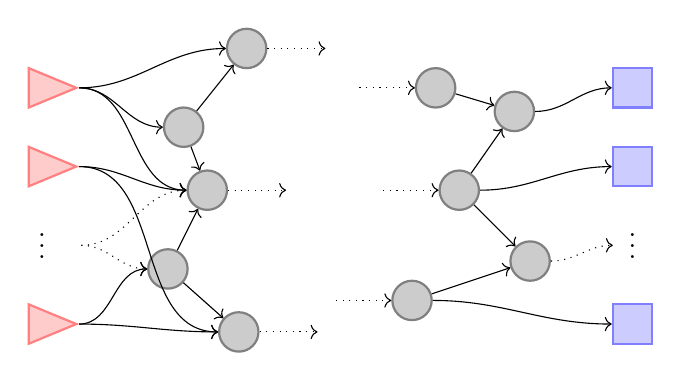
\begin{tikzpicture}
	[%
	input/.style ={isosceles triangle,	draw=red!50,		fill=red!20,		thick,	inner sep=0pt,	minimum size=5mm},%
	inner/.style ={circle,							draw=black!50,	fill=black!20,	thick,	inner sep=0pt,	minimum size=5mm},%
	output/.style={rectangle,					draw=blue!50,	fill=blue!20,	thick,	inner sep=0pt,	minimum size=5mm},%
	]

	% nodes
	\foreach \i in {0,1,3} \node (input\i) at (0,2.5-\i) [input] {};
	
	\node (inner0) at (1.6, 0.2) [inner] {};
	\node (inner1) at (1.8, 2.0) [inner] {};
	\node (inner2) at (2.1, 1.2) [inner] {};
	\node (inner3) at (2.5,-0.6) [inner] {};
	\node (inner4) at (2.6, 3.0) [inner] {};

	\node (inner5) at (4.7,-0.2) [inner] {};	
	\node (inner6) at (5.0, 2.5) [inner] {};
	\node (inner7) at (5.3, 1.2) [inner] {};
	\node (inner8) at (6.0, 2.2) [inner] {};
	\node (inner9) at (6.2, 0.3) [inner] {};	
	
	\foreach \i in {0,1,3} \node (output\i) at (7.5,2.5-\i) [output] {};
	
	% interconnections
	\draw [->] (input0) to [out=0,in=180] (inner1);	
	\draw [->] (input0) to [out=0,in=180] (inner2);	
	\draw [->] (input0) to [out=0,in=180] (inner4);	
	\draw [->] (input1) to [out=0,in=180] (inner2);	
	\draw [->] (input1) to [out=0,in=180] (inner3);	
	\draw [dotted, ->] (0.5,0.5)  to [out=0,in=180] (inner0);	
	\draw [dotted, ->] (0.5,0.5)  to [out=0,in=180] (inner2);	
	\draw [->] (input3) to [out=0,in=180] (inner0);	
	\draw [->] (input3) to [out=0,in=180] (inner3);	
	
	\draw [->] (inner0) to (inner3);
	\draw [->] (inner0) to (inner2);
	\draw [->] (inner1) to (inner2);
	\draw [->] (inner1) to (inner4);
	
	\draw [dotted, ->] (inner2) to +(0:1);
	\draw [dotted, ->] (inner3) to +(0:1);
	\draw [dotted, ->] (inner4) to +(0:1);
	
	\draw [dotted, <-] (inner5) to +(180:1);
	\draw [dotted, <-] (inner6) to +(180:1);
	\draw [dotted, <-] (inner7) to +(180:1);
	
	\draw [->] (inner5) to (inner9);	
	\draw [->] (inner6) to (inner8);
	\draw [->] (inner7) to (inner8);
	\draw [->] (inner7) to (inner9);
	
	\draw [->] (inner5) to [out=0,in=180] (output3);
	\draw [->] (inner7) to [out=0,in=180] (output1);
%	\draw [dotted,->] (inner7) to [out=0,in=180] (7.25,0.5);	
	\draw [->] (inner8) to [out=0,in=180] (output0);
%	\draw [->] (inner8) to [out=0,in=180] (output1);
	\draw [dotted,->] (inner9) to [out=0,in=180] (7.25,0.5);	
%	\draw [->] (inner9) to [out=0,in=180] (output3);
	
	\foreach \i in {0,7.5} \node at (\i,0.6) {$\vdots$};
	
\end{tikzpicture}
	\caption{	Generic scheme of a neural network. %
						Triangles (red) are input nodes, circles (grey) are inner nodes, and squares (blue) are output nodes. %
						Interconnections among nodes are represented by arrows: %
						continuous when both elements are drawn, and dotted otherwise.
						%						I chose a non-standard representation to emphasize the nonlinear nodes, which will use a nonlinear activation function. %
						}
	\label{fig:generic_NN}
\end{figure}

Nodes can all implement the same function or behave differntly, depending on the type of neural network.
%Each node can operate in the same way of the others or in a completely different manner, depending on the type of neural network.
The operation of nodes resembles that of animal neurons: various input gets collected and elaborated together to obtain an output, which will become one of the many inputs for subsequent neurons/nodes.
Specifically, the most used model for neurons is the McCulloch–Pitts (MCP) neuron.
It is divided into two parts, as shown in \autoref{fig:generic_node}: the first part is a weighted sum of the inputs, while the second part is given by the so called activation function.
\newpage
\begin{figure}[ht]
	\centering
	\tikzsetnextfilename{GenericNode}
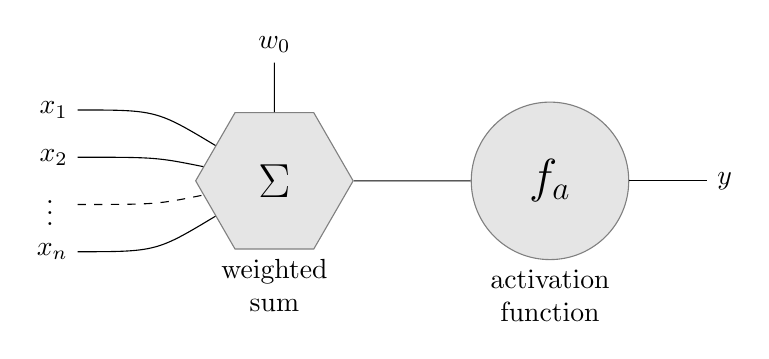
\begin{tikzpicture}
	\node [shape=circle, minimum size=2cm, draw=gray!100, fill=gray!20]%
				(af) at (1.5,0) {\LARGE $f_a$};
	\node at (af.south) [below, align=center] {activation \\ function};
	\node [regular polygon, regular polygon sides=6, minimum size=2cm, draw=gray!100, fill=gray!20]%
				(ws) at (-2,0) {\LARGE $\Sigma$};
	\node at (ws.south) [below, align=center] {weighted \\ sum};
	\draw (ws) to (af);
	\foreach \i in {1,2,4}	\draw (-4.5,1.5-0.6*\i) .. controls (-3.5,1.5-0.6*\i) .. (ws);
	\draw [dashed] (-4.5,-0.3) node {$\vdots\qquad$} .. controls (-3.5,-0.3) .. (ws);
	\foreach \i in {1,2}		\node at (-4.5,1.5-0.6*\i) [left] {$x_\i$};
	\node at (-4.5,-0.9)  [left] {$x_n$};
	\draw (-2,1.5) node [above] {$w_0$} to (ws);
	\draw (af) to (3.5,0) node [right] {$y$};
\end{tikzpicture}
	\caption{Generic node representation. $x$-values are inputs, $y$-values are outputs, $w_0$ is the bias.}
	\label{fig:generic_node}
\end{figure}
The node is described mathematically by \cref{eq:Generic_node_function}
\begin{equation}
y = f_a \left(  w_0 + \sum_{i=1}^{n} w_i x_i \right),
\label{eq:Generic_node_function}
\end{equation}
where $f_a$ is the activations function, evaluated on the sum of the input $x_i$ weighted with $w_i$, plus a bias $w_0$.

Each node accepts values at its inputs and produces an output accordingly.
However, in addition to the input, the output depends also on the node's parameters: the weights and the bias, which are usually changed outside the operative phase of the neural network (see \autoref{sec:Working_Principles_of_ANNs}).

Moreover it is mandatory for the activation function $f_a\left(\cdot\right)$ to be nonlinear, because otherwise a collection of nodes will result in just a weighted sum of its inputs.
Two examples of nonlinear function are shown below in \autoref{fig:activation_function_examples}.

\begin{figure}[ht]
	\begin{subfigure}[b]{0.49\textwidth}
		\centering
		\tikzsetexternalprefix{tikz/}	% set subfolder
\tikzsetnextfilename{HeavisideThetaFunction}
\begin{tikzpicture}[baseline]
	\begin{axis}[%
%			yticklabel pos=upper,%
			title ={$\Theta(x)$},%
			xlabel={$x$},%
%			ylabel={$\Theta(x)$},%
		]
		\newcommand\LIM{5}
		\addplot [blue, domain=-\LIM:0,	samples=501,]	{0};
		\addplot [blue, domain=0:\LIM,		samples=501,]	{1};
	\end{axis}
\end{tikzpicture}
		\caption{}
		\label{fig:activation_function_example_1}
  \end{subfigure}
  \begin{subfigure}[b]{0.49\textwidth}
  		\centering
		\tikzsetexternalprefix{tikz/}	% set subfolder
\tikzsetnextfilename{LogisticFunction}
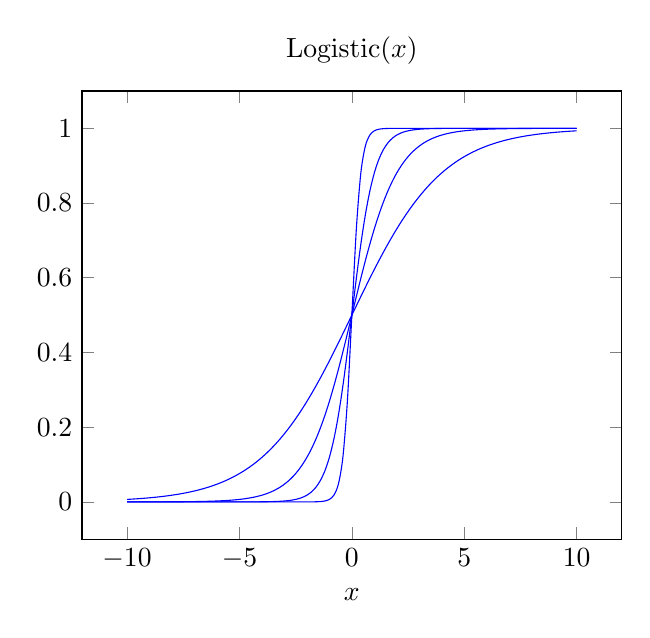
\begin{tikzpicture}[baseline]
	\begin{axis}[%
%			yticklabel pos=upper,%
			title ={$\mathrm{Logistic}(x)$},%
			xlabel={$x$},%
%			ylabel={$\mathrm{Logistic}(x)$},%
		]
		\newcommand\LIM{10}
		\addplot [blue, 	domain=-\LIM:\LIM,		samples=101, smooth,]	{(1+exp(-0.5*x))^-1};
		\addplot [blue, 	domain=-\LIM:\LIM,		samples=101, smooth,]	{(1+exp(-1.0*x))^-1};
		\addplot [blue, 	domain=-\LIM:\LIM,		samples=101, smooth,]	{(1+exp(-2.0*x))^-1};
		\addplot [blue, 	domain=-\LIM:\LIM,		samples=101, smooth,]	{(1+exp(-5.0*x))^-1};
	\end{axis}
\end{tikzpicture}
		\caption{}
		\label{fig:activation_function_example_2}
  \end{subfigure}
  \caption{Examples of activation function: (\ref{fig:activation_function_example_1}) is the well-known step function, or Heaviside $\Theta$, (\ref{fig:activation_function_example_2}) depicts a few functions from the family of the Logistic functions.}
  	\label{fig:activation_function_examples}
\end{figure}

One can distinguish at least three type of nodes in every neural network: input, inner/hidden, and output nodes.
Input nodes take one input value, from the outside of the neural network, and pass it on to the inner nodes unchanged.
Inner/hidden nodes take many inputs and generate an output through the activation function.
Output nodes, similarly to input nodes, take one input value, from the inside of the \acs{ANN}, and pass it on to the outside.

\subsection*{Standard Representation}
%This is not the orthodox description, but I claim that it is more consistent than the standard representation with the idea of functional \textit{black box}, in which input and output are the only visible nodes, while the other are hidden inside.
The way I depicted a generic neuromorphic network in \autoref{fig:generic_NN} is not the standard representation used in books and research papers.
The main difference is that usually weights are commonly represented on the connection between the nodes, which are then designated to apply only the activation function.
Moreover the input layer is linear as it feeds the inner nodes with the input data, while the output layer is actually given by the last nonlinear layer of the inner nodes.
A generic network is shown in \autoref{fig:standardNNdesc}.

\begin{figure}[ht]
	\begin{subfigure}[b]{0.49\textwidth}
		\centering
		\tikzsetnextfilename{standardNNdesc}
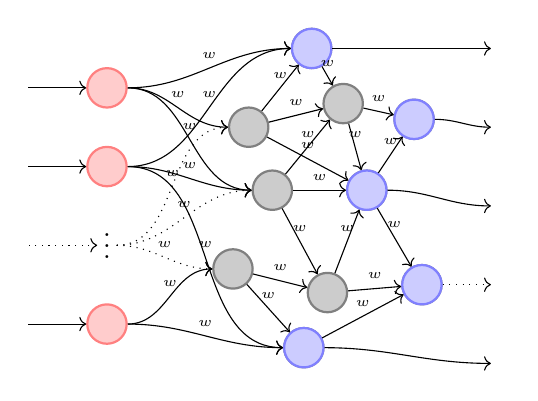
\begin{tikzpicture}
	[%
	input/.style ={circle,	draw=red!50,		fill=red!20,		thick,	inner sep=0pt,	minimum size=5mm},%
	inner/.style ={circle,	draw=black!50,	fill=black!20,	thick,	inner sep=0pt,	minimum size=5mm},%
	outer/.style ={circle,	draw=blue!50,	fill=blue!20,	thick,	inner sep=0pt,	minimum size=5mm},%
	]

	\newcommand\lin{0}
	\newcommand{\lout}{5}
	
	% nodes
	% input
	\foreach \i in {0,2,3} \node (input\i) at (\lin,0.5+\i) [input] {};
	\node (input1)		at (\lin,1.5) {}; 		\node at (\lin,1.6) {$\vdots$};
	% inner
	\foreach \n/\x/\y in {	0/1.6/1.2, 1/1.8/3.0, 2/2.1/2.2, 5/2.8/0.9, 6/3.0/3.3, %
												3/2.5/0.2, 4/2.6/4.0, 7/3.3/2.2, 8/3.9/3.1, 9/4.0/1.0 %
												}
			\node (inner\n) at (\x,\y) [inner] {};
	% outer
	\foreach \n/\x/\y in {	3/2.5/0.2, 4/2.6/4.0, 7/3.3/2.2, 8/3.9/3.1, 9/4.0/1.0 }
			\node (outer\n) at (\x,\y) [outer] {};
	% output
	\foreach \i in {0,1,2,3,4} \node (output\i) at (\lout,\i) {};
	
	% interconnections
	% to input
	\foreach \i/\type in {0/solid, 1/dotted, 2/solid, 3/solid}
		\draw [<-, \type] (input\i) -- ++(-1,0);
	
	% input to inner
	\foreach \i/\o in {0/0, 0/3, 2/2, 2/3, 2/4, 3/1, 3/2, 3/4}
		\draw [->] (input\i) to [out=0,in=180] node [midway, above] {\tiny{ $w$ } } (inner\o);
		
	\foreach \i/\o in {1/0, 1/1, 1/2}
		\draw [dotted, ->] (input\i) to [out=0,in=180] node [midway, above] {\tiny{ $w$ } } (inner\o);

	% inner to inner
%	\node at (0,0) {ciao};
	\foreach \i/\o in {	0/3, 0/5, 1/4, 1/6, 1/7, 2/5, 2/6, 2/7, %
											3/9, 4/6, 5/7, 5/9, 6/7, 6/8, 7/8, 7/9}
		\draw [->] (inner\i) -- (inner\o) node [midway, above] {\tiny{ $w$ } };
	
	% outer to output	
	\foreach \i/\o in {3/0, 7/2, 8/3, 4/4}
		\draw [->] (outer\i) to [out=0,in=180] (output\o);
				
	\foreach \i/\o in {9/1}
		\draw [dotted, ->] (outer\i) to [out=0,in=180] (output\o);
	
\end{tikzpicture}
		\caption{Standard way of representing networks}
		\label{fig:standardNNdesc}
  \end{subfigure}
  \begin{subfigure}[b]{0.49\textwidth}
  		\centering
		\tikzsetnextfilename{BlackBoxNN}
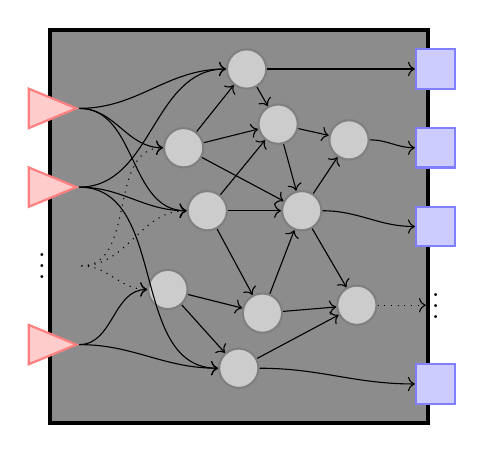
\begin{tikzpicture}
	[%
	input/.style ={isosceles triangle,	draw=red!50,		fill=red!20,		thick,	inner sep=0pt,	minimum size=5mm},%
	inner/.style ={circle,							draw=black!50,	fill=black!20,	thick,	inner sep=0pt,	minimum size=5mm},%
	output/.style={rectangle,					draw=blue!50,	fill=blue!20,	thick,	inner sep=0pt,	minimum size=5mm},%
	]

	\newcommand\lin{0}
	\newcommand{\lout}{5}
	
	% black box
	\filldraw [thick, draw=black, fill=gray!90, line width=0.5mm] (0.1,-1.5) rectangle (4.9,3.5);	
	
	% nodes
	\foreach \i in {0,1,3} \node (input\i) at (\lin,2.5-\i) [input] {};
	
	\foreach \i in {0,1,2,4} \node (output\i) at (\lout,3-\i) [output] {};
	
	\node (inner0) at (1.6, 0.2) [inner] {};
	\node (inner1) at (1.8, 2.0) [inner] {};
	\node (inner2) at (2.1, 1.2) [inner] {};
	\node (inner3) at (2.5,-0.8) [inner] {};
	\node (inner4) at (2.6, 3.0) [inner] {};

	\node (inner5) at (2.8,-0.1) [inner] {};
	\node (inner6) at (3.0, 2.3) [inner] {};
	\node (inner7) at (3.3, 1.2) [inner] {};
	\node (inner8) at (3.9, 2.1) [inner] {};
	\node (inner9) at (4.0, 0.0) [inner] {};
	
	\node (input2)		at (\lin,0.5) {}; 		\node at (\lin,0.6) {$\vdots$};
	\node (output3)	at (\lout,0.0) {}; 	\node at (\lout,0.1) {$\vdots$};
	
	% interconnections
	\draw [->] (input0) to [out=0,in=180] (inner1);
	\draw [->] (input0) to [out=0,in=180] (inner2);
	\draw [->] (input0) to [out=0,in=180] (inner4);
	\draw [->] (input1) to [out=0,in=180] (inner2);
	\draw [->] (input1) to [out=0,in=180] (inner3);
	\draw [->] (input1) to [out=0,in=180] (inner4);
	\draw [dotted, ->] (0.5,0.5)  to [out=0,in=180] (inner0);
	\draw [dotted, ->] (0.5,0.5)  to [out=0,in=180] (inner1);
	\draw [dotted, ->] (0.5,0.5)  to [out=0,in=180] (inner2);
	\draw [->] (input3) to [out=0,in=180] (inner0);
	\draw [->] (input3) to [out=0,in=180] (inner3);
	
	\draw [->] (inner0) to (inner3);
	\draw [->] (inner0) to (inner5);
	\draw [->] (inner1) to (inner4);
	\draw [->] (inner1) to (inner6);
	\draw [->] (inner1) to (inner7);
	\draw [->] (inner2) to (inner5);
	\draw [->] (inner2) to (inner6);
	\draw [->] (inner2) to (inner7);
	\draw [->] (inner3) to (inner9);
	\draw [->] (inner4) to (inner6);
	\draw [->] (inner5) to (inner7);
	\draw [->] (inner5) to (inner9);
	\draw [->] (inner6) to (inner7);
	\draw [->] (inner6) to (inner8);
	\draw [->] (inner7) to (inner8);
	\draw [->] (inner7) to (inner9);
	
	\draw [->] (inner4)  to [out=0,in=180] (output0);
	\draw [->] (inner8)  to [out=0,in=180] (output1);
	\draw [->] (inner7)  to [out=0,in=180] (output2);
	\draw [dotted, ->] (inner9)  to [out=0,in=180] (output3);
	\draw [->] (inner3)  to [out=0,in=180] (output4);
	
\end{tikzpicture}
		\caption{Representation of the black-box concept}
		\label{fig:black_box_NN}
  \end{subfigure}
  \caption{}
  	\label{fig:description_comparison}
\end{figure}

On the contrary, I consider the inner nodes as the only place where any kind of elaboration on the data happens.
Inner nodes have a number of inputs, which are weighted and summed together to be entered as argument in the activation function.
This leads to a natural separation between input/output nodes, which acquire the task of providing data from/to the outside, and inner nodes, which is where the activation function and/or the weighted sum are carried out.

This non-standard description, moreover, is consistent with the idea of functional \textit{black box}, in which input and output are the only visible nodes, while the other are hidden inside, as shown in \autoref{fig:generic_NN}.
%Therefore I can easily distinguish the nodes which will use a nonlinear activation function.
%Questa non è la visione standard/ortodossa, ma è consistente con un'idea di 'black box' in cui gli input e output sono gli unici nodi visibili. mentre gli altri sono all'interno della scatola nera.

\subsection{Applications of ANNs}
\label{ssec:Applications_of_ANNs}
Conventional computers are extremely fast and efficient in executing simple algebraic tasks and they can perform more complex activities if provided with the correct series of instructions.
Hence algorithms can solve arbitrary difficult problems, provided that the necessary steps are know.

Artificial neural networks take a different path in the solution of a given problem.
\acsp{ANN} cannot be programmed, but they learn from the examples that are provided to them.
Then they exploit their internal complexity to minimize the error and hence automatically solve the problem.
After a network has been prepared, it is able to operate much faster than the complex algorithms on conventional computers.

\acsp{ANN} have proven to be extremely good at recognize patterns, which can be used to solve problems in several classes.
For example, classification problems are solved by the recognition of attributes of the input element.
Likewise, clustering is obtained when a sequence of examples is grouped according to their features.
Moreover, regression analysis and time series prediction can be obtained, when a sequence of data is fed to the network.
% Regression: Predicting a continuous variable\\
% Classification: Predicting a variable with finite possible values\\
% Clustering: Grouping data\\
% https://cs.stackexchange.com/questions/58131/are-neural-networks-a-type-of-reinforcement-learning-or-are-they-different

\section{Working Principles of ANNs}
\label{sec:Working_Principles_of_ANNs}
Because of its topology, each neural network will behave in a different manner from other neural networks with diverse, or even similar, arrangements of nodes.
Moreover the same neural network will perform a certain task better or worse also depending on how inputs are weighted at each hidden node, and normally those parameters are initialized with a random value at the creation of the network.
For this reason, before a neural network is considered ready to perform a task, it usually must go through three training stages: learning phase, validation phase, and testing phase.
Every one of these stages is meant to prepare the network to work as required from the designer.

\subsection{Learning Process}
\label{ssec:Learning_Process}
During the learning process the neural network is run on a set of known inputs $x$, each paired with its correct answer $y$, or target, in a second set of data.
The neural network will produce at the output a third set $\hat{y}$, which should be as close as possible to the correct answers, when the network works properly.
%However this happens rarely, if ever, and a change in the way data is elaborated becomes necessary.
%The usual \ref{} way is to keep the same topology, but tweak the weights that connect the hidden nodes together.
%On account of this need, one have to quantify the distance of the predicted result of the artificial neural network from the correct answer.
%This is made by means of the loss function.
Typically weights among nodes are initialized randomly and the distance of the network outcome from the target function is measured through a loss function.
Then weights are modified in order to decrease the loss function to its lowest possible value. %up to a tolerance limit is achieved.

\subsubsection{Loss function}
\label{sssec:Loss_function}
The loss function $L(y, \hat{y})$ evaluates the difference between the predicted and the correct answer.
Usually, this quantity is linked to the geometrical distance between the predicted output and the target $\left| \hat{y}-y \right|$.

The most common loss function is the \acfi{MSE}.
Assuming to have an input set of $N$ examples paired with the same number of targets, and that the outputs and the targets are composed by $C$ values, or classes, the function becomes:
\begin{equation}
	L(y, \hat{y}) = f_{MSE}(y, \hat{y}) = \frac{1}{N} \sum_{n=1}^N \sum_{i=1}^C \left( \hat{y}_{n,i} - y_{n,i} \right)^2,
\end{equation}
where each example in the set is subtracted to its target and then squared.
Finally the mean of all squares gives the expected result.

Another commonly used function is the \acfi{CEL} (also known as negative log likelihood),
\begin{equation}
	L(y, \hat{y}) = f_{CEL}(y, \hat{y}) = - \frac{1}{N} \sum_{n=1}^N \sum_{i=1}^C y_{n,i} \log \left( \hat{y}_{n,i} \right),
\end{equation}
which expects positive values at the input.
Hence the error $-y\log \left( \hat{y} \right)$, quantified for each element in each example, is always a positive number.
The mean over all examples in the set returns the results.

Alternatively, variations of the previous methods are given by taking the sum of the examples in place of the mean, or by calculating a loss function for each example instead of evaluating it for the whole set.

Depending on the class of the problem, e.g. classification or image recognition, a different loss function is chosen.
In fact, since the loss function drives the weights update process, it is important to choose the correct one.

\subsubsection{Weights Update Process}
\label{sssec:Weights_Update_Process}

The weights update process is a difficult task, and probably the most computationally expensive one in running a neural network.
There is a variety of methods to chose from, depending on the type of artificial network and the resources available.

A widely used algorithm is the gradient descent, from its most simple version to more complex variations such as \acfi{SGD}.
This method updates the weights by subtracting a value proportional to the gradient of the loss function in respect to the weights themselves times a positive factor called \textit{learning rate}, as shown below.
\begin{equation}
	\left.w_i\right|_{n+1} = \left.w_i\right|_n - lr \cdot \frac{\partial L}{\partial \left.w_i\right|_n}
\end{equation}
where $\left.w_i\right|_{n}$ are the current weights, $lr$ is the learning rate, $\dfrac{\partial L}{\partial \left.w_i\right|_n}$ is the first derivative of the loss function in respect to the i-th weight at the current step, and $\left.w_i\right|_{n+1}$ are the updated weights.
%Hence it is necessary to calculate the gradient $\bigtriangledown_w L$.
This method is equivalent to minimize the error on the loss function, by following the gradient $\bigtriangledown_w L$.
This vector lives in the multidimensional space of the loss function $L:\mathbb{R}^W \mapsto \mathbb{R}$, where $W$ is the total number of parameters in the network.

The most used algorithm is called \textit{backpropagation}: it computes the first derivative of the loss function $L$ in respect to all the parameters of the network, the weights, starting from the end of the artificial network and going backward toward the input, hence the name backpropagation.
Since the number of connections between nodes might be even order of magnitude bigger than the number of nodes, it is simple to understand how large networks are computationally expensive to train.

In early days, this algorithm was used together with the Logistic activation function.
Due to the saturating behavior of the function, the gradient is repeatedly multiplied by small values at each layer.
Hence, the effect of backpropagation becomes negligible for the first layer on deep networks
This problem is known as \textit{vanishing gradient} problem.
Thanks to the introduction of non saturating activation functions, the training of deep neural network has become gradually possible \cite{krizhevsky2012imagenet}.
%\paragraph{Other types of learning processes} are used, e.g. unsupervised/reinforced.

\subsection{Validation Process}
\label{ssec:Validation_Process}
The validation process is carried out at the same time of the training process and consists on testing the neural network on a new set of examples.
Differently from the learning process, during validation the output predicted by the network are compared to the examples, but the weights are not updated.
Instead, the loss function is used as a control parameter to prevent overfitting

Overfitting is the phenomenon in which a neural network recognizes specific features of the samples instead of the more general ones.
It occurs when the network is trained over and over on the same set of data.
Since the specific features are the ones that characterize precisely the test dataset, they should not characterize other dataset.
Therefore, by periodically testing the network on a novel set, i.e. the validation set which is different from the training set, one can avoid or at least reduce the problem.

The validation process happens repeatedly throughout the training process, more or less often, depending on the resources available and the size of the dataset.

\subsection{Testing Process}
\label{ssec:Testing_Process}
At the end of the training and validation processes, there is the process of testing the artificial neural network.
The network is tested on a new set of data, the test data.
This time the predicted outputs are compared to the correct answers, but no weights are changed.
Instead, an overall value of the correctness is evaluated and it is often expressed in percentage.

\begin{figure}[htbp]
	\centering
	\tikzsetexternalprefix{tikz/}	% set subfolder
\tikzsetnextfilename{LVTcurves}
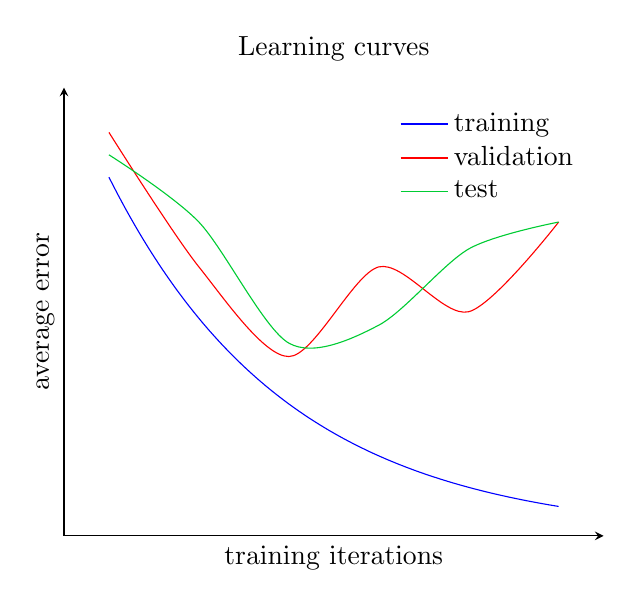
\begin{tikzpicture}[baseline]
	\begin{axis}[
			title ={Learning curves},
			xlabel={training iterations},
			ylabel={average error},
			axis x line=bottom,
			axis y line=left,
			domain=0:5,
			xmin=-0.5, xmax=5.5,
			ymin=0,	ymax=1,
			ticks=none,
			legend style={draw=none},
			legend pos= north east,
			legend entries={training,validation,test},
			legend cell align=left,
		]

		\addplot [blue, samples=101, smooth]	{.8*exp(-0.5*x)};
		
		\addplot [red, smooth] coordinates {
			(0.0,0.9)
			(1.0,0.6)
			(2.0,0.4)
			(3.0,0.6)
			(4.0,0.5)
			(5.0,0.7)
		};
		
		\addplot [green!80!blue, smooth] coordinates {
			(0.0,0.85)
			(1.0,0.7)
			(2.0,0.43)
			(3.0,0.47)
			(4.0,0.64)
			(5.0,0.7)
		};
		
%		\addplot [black, only marks, mark=o] coordinates {(2.0,0.4)}
		
	\end{axis}
\end{tikzpicture}
	\caption{The learning curves are the value of the loss function, or criterion, as a function of the training iterations.
	Both the validation and the test error are usually higher than the errors on the training set.
	Sometimes, to avoid overfitting, the training procedure is stopped at a minimum of the validation learning curve \cite{duda2012pattern}.
	}
	\label{fig:LVTcurves}
\end{figure}

\subsection{Datasets}
\label{ssec:Datasets}
Creating a dataset and splitting it into subsets is another problem to deal with.
It is not so simple and straightforward as it appears.
For example a dataset which is too big will lead to a longer training time for the network, whereas a too little set will cause a poor training.

The most naive division is in three equal parts, since three are the phases of preparation for any artificial neural network.
However, as shown later in \autoref{ssec:PyDataset}, when the resources dictates otherwise, other subdivision can be implemented.
In my case, the decision was to follow the suggestions of the authors of the dataset and divide the examples into a training set and a test set only, with a ratio between the two close to 50\%.

\section{Feedforward NN}
\label{sec:Feedforward_NN}

The first and most simple type of neural network is called Feedforward.
In this kind of neural network, nodes are divided into groups called \textit{layers}.
A layer is a collection of nodes that accepts inputs from a preceding group and generate as many outputs as the number of nodes in the layer.
Each layer of a Feedforward neural network is connected in series with the others, except for the input layer at the beginning and the output layer at the end.
As for the single nodes, the inner layer are called hidden, because usually not accessible.

The information travels from the input to the output and gets elaborated from each hidden layer: there are neither connection between nodes of the same layer, nor loops or feedback between layers.
%Depending on the topology of the network, there might be more or less layers, each composed by the same or a different number of nodes.
The number of hidden layers and the number of nodes they contain depends on the network topology.
Moreover the connection between the layers might be complete, i.e. each node in the layer accepts each input of the preceding layer, in that case the layer is said to be \textit{fully connected}, or sparse as in the case of convolutional layers (see \autoref{par:Convolutional}).

\subsection{Perceptron}
\label{ssec:Perceptron}

The most naive topology of a Feedforward neural network is given by the so called \textit{Perceptron}.
The Perceptron dates back to the 1957, when the homonym \textit{Perceptron algorithm} was software implemented by Frank Rosenblatt on a computer (IBM 704) and only subsequently in hardware as the \textit{Mark 1 perceptron} \cite{frank1957perceptron,Rosenblatt1958}.
The graph of a generic (single layer) perceptron \acs{ANN} is shown in \autoref{fig:Perceptron}.

\begin{figure}[ht]
	\centering
	\tikzsetnextfilename{PerceptronNN}
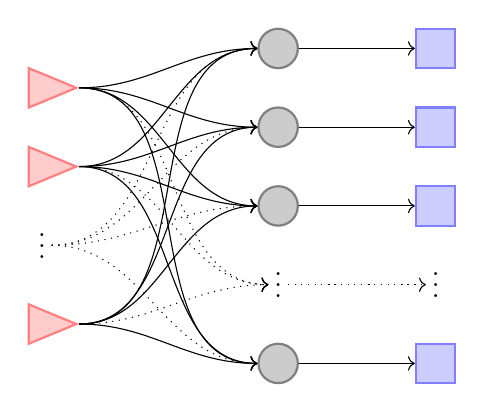
\begin{tikzpicture}
	[%
	input/.style ={isosceles triangle,	draw=red!50,		fill=red!20,		thick,	inner sep=0pt,	minimum size=5mm},%
	inner/.style ={circle,							draw=black!50,	fill=black!20,	thick,	inner sep=0pt,	minimum size=5mm},%
	output/.style={rectangle,					draw=blue!50,	fill=blue!20,	thick,	inner sep=0pt,	minimum size=5mm},%
	]

	\newcommand\lin{0}
	\newcommand{\lhid}{3}
	\newcommand{\lout}{5}
	
	% nodes
	\foreach \i in {0,1,3} \node (input\i) at (\lin,2.5-\i) [input] {};
	
	\foreach \i in {0,1,2,4} \node (inner\i) at (\lhid,3-\i) [inner] {};
	
	\foreach \i in {0,1,2,4} \node (output\i) at (\lout,3-\i) [output] {};
	
	\node (input2)		at (\lin,0.5) {}; 		\node at (\lin,0.6) {$\vdots$};
	\node (inner3)		at (\lhid,0.0) {}; 	\node at (\lhid,0.1) {$\vdots$};
	\node (output3)	at (\lout,0.0) {}; 	\node at (\lout,0.1) {$\vdots$};
	
	% interconnections
	\foreach \i in {0,1,3}%
		\foreach \j in {0,1,2,4}%
			\draw [->] (input\i) to [out=0, in=180] (inner\j);
	
	\foreach \i in {0,1,3}%
		\draw [dotted, ->] (input\i)	to [out=0, in=180] (inner3);
	\foreach \j in {0,1,2,4}%
		\draw [dotted, ->] (input2) 	to [out=0, in=180] (inner\j);
	\foreach \i in {0,1,2,4}%
		\draw [->] (inner\i) to [out=0, in=180] (output\i);
	\draw [dotted, ->] (inner3) to [out=0, in=180] (output3);
	
\end{tikzpicture}
	\caption{%
		Perceptron type neural network: in this representation the perceptron has $n$ inputs and $m$ outputs as well as a hidden layer with $m$ nodes. %
%		Colors, shape and styles are the same as in \autoref{fig:generic_NN} \vpageref{fig:generic_NN}.%
		}
	\label{fig:Perceptron}
\end{figure}

By adding more than one hidden perceptron layer to the neural network, one obtain the so called \acfi{MLP}.
This allows for more computational complexity, e.g. \acs{MLP} can solve the \acs{XOR} problem, whereas single layer perceptron cannot \ref{}.
When the number of hidden layers is more than two, the network is called \textit{deep}.
A deep \acs{MLP} is shown in \autoref{fig:deepMLP}.

\begin{figure}[ht]
	\centering
	\tikzsetnextfilename{MLPNN}
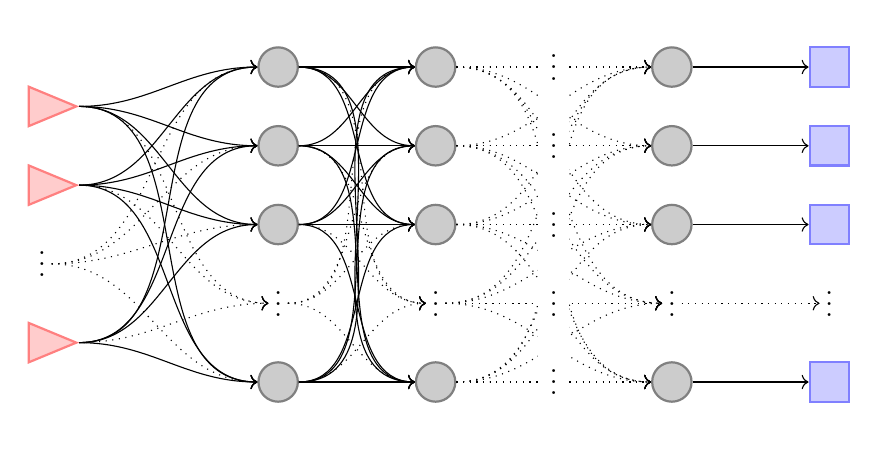
\begin{tikzpicture}
	[%
	input/.style ={isosceles triangle,	draw=red!50,		fill=red!20,		thick,	inner sep=0pt,	minimum size=5mm},%
	inner/.style ={circle,							draw=black!50,	fill=black!20,	thick,	inner sep=0pt,	minimum size=5mm},%
	output/.style={rectangle,					draw=blue!50,	fill=blue!20,	thick,	inner sep=0pt,	minimum size=5mm},%
	]

	\newcommand\lin{0}
	\newcommand{\lhid}{3}
	\newcommand{\lhidb}{5}
	\newcommand{\lhidc}{6.5}
	\newcommand{\lhidd}{8}
	\newcommand{\lout}{10}
	
	% nodes
	\foreach \i in {0,1,3} \node (input\i) at (\lin,2.5-\i) [input] {};
	
	\foreach \j in {\lhid,\lhidb,\lhidd}%
		\foreach \i in {0,1,2,4} \node (inner\j_\i) at (\j,3-\i) [inner] {};
	
	\foreach \i in {0,1,2,4} \node (output\i) at (\lout,3-\i) [output] {};
	
	\node (input2)		at (\lin,0.5) {}; 		\node at (\lin,0.6) {$\vdots$};
	\foreach \j in {\lhid,\lhidb,\lhidd}%
		\node (inner\j_3)		at (\j,0.0) {};
	\foreach \j in {\lhid,\lhidb,\lhidd}%
		\node at (\j,0.1) {$\vdots$};
	\node (output3)	at (\lout,0.0) {}; 	\node at (\lout,0.1) {$\vdots$};
	
	% interconnections
	% in - hid1
	\foreach \i in {0,1,3}%
		\foreach \j in {0,1,2,4}%
			\draw [->] (input\i) to [out=0, in=180] (inner\lhid_\j);
	\foreach \i in {0,1,3}%
		\draw [dotted, ->] (input\i)	to [out=0, in=180] (inner\lhid_3);
	\foreach \j in {0,1,2,4}%
		\draw [dotted, ->] (input2) 	to [out=0, in=180] (inner\lhid_\j);
	
	\foreach \i in {0,1,2,4}%
		\foreach \j in {0,1,2,4}%
			\draw [->] (inner\lhid_\i) to [out=0, in=180] (inner\lhidb_\j);
	\foreach \i in {0,1,2,4}%
		\draw [dotted, ->] (inner\lhid_\i)	to [out=0, in=180] (inner\lhidb_3);
	\foreach \j in {0,1,2,4}%
		\draw [dotted, ->] (inner\lhid_3) to [out=0, in=180] (inner\lhidb_\j);
	
	\foreach \i in {0,1,2,3,4}%
		\foreach \j in {0,1,2,3,4}%
			\draw [dotted,->] (inner\lhidb_\i) to [out=0, in=180] (inner\lhidd_\j);
	\fill [white] (6.3,-1.5) rectangle (6.7,3.5);
	\foreach \i in {-0.9,0.1,1.1,2.1,3.1}%
		\node at (\lhidc,\i) {$\vdots$};

	\foreach \i in {0,1,2,4}%
		\draw [->] (inner\lhidd_\i) to [out=0, in=180] (output\i);

	\draw [dotted, ->] (inner\lhidd_3) to [out=0, in=180] (output3);
	
\end{tikzpicture}
	\caption{	Deep \acf{MLP}, fully connected.}
	\label{fig:deepMLP}
\end{figure}

In principle any shape is possible, i.e. each layer could have a different number of nodes, however often the layers at the beginning are wider than the layer at the end of the network (see following section).
Moreover, in literature with the term perceptron one almost always refers to fully connected feedforward networks \ref{}.

\subsection{Other Feedforward NNs}
\label{ssec:Other_Feedforward_NNs}

Feedforward neural networks are a large family that includes many other types besides the perceptron one.
A few names are autoencoder, time delay, and convolutional neural networks.
Autoencoders \acsp{ANN} are feedforward networks with the same number of input and output nodes, with the purpose of reconstructing its own inputs.
For this reason autoencoders employ unsupervised learning.
Time delay networks have a feedforward structure and their purpose is to analyze patterns in

\subsubsection{Convolutional Neural Networks}
\label{par:Convolutional}
\acp{CNN} are inspired to the visual cortex, in which neurons are not fully connected all the inputs but only to a restricted region.
\aclp{CNN} are a type of feedforward network conceived to recognize images without being misled by distortions such as translation, skewing, or scaling.
Its input is often represented as a 2D matrix, instead of a 1D vector.
This kind of network is usually composed by many layers: the most recurring is prevalent the convolutional one, but other types can be mixed together too.

\begin{figure}[ht]
	\centering
	\tikzsetnextfilename{ConvNN}
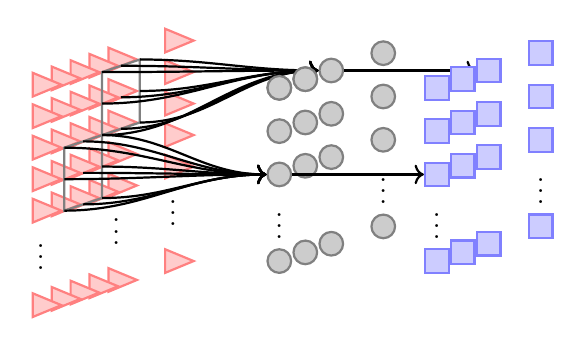
\begin{tikzpicture}[
		baseline,
		input/.style ={isosceles triangle,	draw=red!50,		fill=red!20,		thick,	inner sep=0pt,	minimum size=3mm},
		inner/.style ={circle,							draw=black!50,	fill=black!20,	thick,	inner sep=0pt,	minimum size=3mm},
		output/.style={rectangle,					draw=blue!50,	fill=blue!20,	thick,	inner sep=0pt,	minimum size=3mm},
	]

	\newcommand\lin{0}
	\newcommand{\lhid}{3}
	\newcommand{\lout}{5}
	
	%	vdots
	\foreach \x in {0,3,7}
			\node at (\lin-0.4*0.6*\x,0.4*1.8-0.4*0.2*\x) {$\vdots$};
	\foreach \z in {\lhid, \lout}
		\foreach \x in {1,5}
				\node at (\z-0.55*0.6*\x,0.55*2.0-0.55*0.2*\x) {$\vdots$};
	
	% nodes
	\foreach \x/\xt in {0/n,3,4,5,6,7}
		\foreach \y/\yt in {0/n,3,4,5,6,7}
			\node [input] (input\xt_\yt) at (\lin-0.4*0.6*\x,0.4*\y-0.4*0.2*\x) {};
	
	\foreach \x/\xt in {1/n,3,4,5}
		\foreach \y/\yt in {1/n,3,4,5}
			\node [inner] (inner\xt_\yt) at (\lhid-0.55*0.6*\x,0.55*\y-0.55*0.2*\x) {};
			
	\foreach \x/\xt in {1/n,3,4,5}
		\foreach \y/\yt in {1/n,3,4,5}
			\node [output] (output\xt_\yt) at (\lout-0.55*0.6*\x,0.55*\y-0.55*0.2*\x) {};
	
	% interconnections

	\draw [black!50,thick] (input3_5.east) -- (input5_5.east)%
		-- (input5_7.east) -- (input3_7.east) -- cycle;
%	\draw [black!50,thick] (input4_4.east) -- (input4_6.east)%
%		-- (input6_6.east) -- (input6_4.east) -- cycle;
	\draw [black!50,thick] (input5_3.east) -- (input5_5.east)%
		-- (input7_5.east) -- (input7_3.east) -- cycle;	
	
	\foreach \xt in {3,4,5}
		\foreach \yt in {5,6,7}
			\draw [thick,->] (input\xt_\yt)	to [out=0, in=180] (inner3_5);	
	
%	\foreach \xt in {4,5,6}
%		\foreach \yt in {4,5,6}
%			\draw [thick,->] (input\xt_\yt)	to [out=0, in=180] (inner4_4);

	\foreach \xt in {5,6,7}
		\foreach \yt in {3,4,5}
			\draw [thick,->] (input\xt_\yt)	to [out=0, in=180] (inner5_3);
		
	%orange!80!red
	%green!90!blue
	\draw [thick,->] (inner5_3) to [out=0, in=180] (output5_3);
	\draw [thick,->] (inner3_5) to [out=0, in=180] (output3_5);
		
	% redraw some things
	
	\node [inner] at (inner5_5) {};
	\node [inner] at (inner4_5) {};
	\node [output] at (output5_5) {};
	\node [output] at (output4_5) {};
	
\end{tikzpicture}
	\caption{%
		Pictorial representation of a layer of a convolutional supernode.
		Several supernodes might be placed side by side to form a convolutional layer.
		Each node acts on a restricted region of the inputs: in this examples a $3\times 3$ region.
		}
	\label{fig:convolutionalNN}
\end{figure}

This layer performs a two-dimensional convolution over the input matrix of a second 2D matrix of weights, called \textit{feature map}.
Thus, each node of the layer operates on a restricted region to understand if a feature is present or not.
The operating regions are commonly overlapping and the feature map is shared among the nodes in the same layer.
Due to the specific operation of convolutional layers, the number of nodes per layer decreased with each layer.

\aclp{CNN} are nowadays widely used in image recognition with outstanding results and they improve with a steady pace.
A technological application of this kind of network is the real time recognition of obstacles in a vehicle path, for safety and automation purposes in the automotive industry.

\subsection{Other Types of NNs}
\label{ssec:Other_Types_of_NNs}
By changing the topology of the nodes distribution and their connections, one obtain other networks that cannot be catalogued under the class of feedforward networks.
Moreover, those different types of network are not a niche, but they are widely studied as a different approaches to the same or additional problems.

\subsubsection{Recurrent NN}
\label{sssec:Recurrent_NN}
\acp{RNN} are a kind of network in which a portion of the input of nodes depends on the (past) output of the same nodes or nodes of subsequent layers.
That is information does not propagates only forward like in the feedforward networks, but can propagate also backward, for example in loops or in feedbacks.

\begin{figure}[ht]
	\centering
	\tikzsetnextfilename{RecurrentNN}
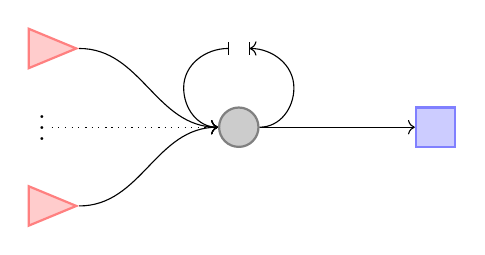
\begin{tikzpicture}[
		baseline,
		input/.style ={
			isosceles triangle,	draw=red!50,		fill=red!20,	
			thick,	inner sep=0pt,	minimum size=5mm
		},
		inner/.style ={
			circle,							draw=black!50,	fill=black!20,
			thick,	inner sep=0pt,	minimum size=5mm
		},
		output/.style={
			rectangle,						draw=blue!50,	fill=blue!20,
			thick,	inner sep=0pt,	minimum size=5mm
		},
	]

	\newcommand\lin{0}
	\newcommand{\lhid}{2.5}
	\newcommand{\lout}{5}
	
	% nodes
	\foreach \i in {0,2} \node (input\i) at (\lin,1-\i) [input] {};
	\node (input1)		at (\lin, 0) {}; 		\node at (\lin, 0.1) {$\vdots$};
	
	\node (inner1) at (\lhid, 0) [inner] {};
	
	\node (output1) at (\lout, 0) [output] {};
	
	% interconnections
	\foreach \i in {0,2}%
		\draw [->] (input\i) to [out=0, in=180] (inner1);
	\draw [dotted, ->] (input1)	to [out=0, in=180] (inner1);
	
	\node (delay) at (\lhid, 1) {};
	\draw [->|] (inner1) to [out=  0, in=270] +(0.7,0.5)   to [out= 90, in=  0] (delay);
	\draw [|->] (delay)  to [out=180, in= 90] +(-0.7,-0.5) to [out=270, in=180] (inner1);
	
	\draw [->] (inner1) to [out=0, in=180] (output1);
	
\end{tikzpicture}
	\caption{%
		Representation of a recurrent node.
		One of the inputs is given by the output itself.
		This output to input connection could be mediated by a delay device, so that for example the output at $t-1$ becomes the input at $t$.
		Depending on the structure of the network, there might be recurrent nodes and/or recurrent groups of nodes, i.e. loops.
		}
	\label{fig:RecurrentNN}
\end{figure}

Recurrent networks have found greatest use in time series analysis and prediction \cite{duda2012pattern}.
However often recurrent type of networks are employed to obtain the same classification of feedforward ones.
In this case, the former are equivalent to the latter, if ``unfolded'' in time.
That is the expansion of the recurrent architecture in time is the same as the topology of the feedforward one in space.

\subsubsection{Reservoir NN}
\label{sssec:Reservoir_NN}
Reservoir neural networks, or \ac{RC}, differ from feedforward and recurrent networks in the learning approach.
In fact, the topology of a reservoir network could be exactly the same as that of a deep multi-layer perceptron or that of a recurrent network.
However, the reservoir computing differs in approach in respect to deep learning.
It claims that it is not necessary to learn all the weights of the network, as in deep learning, but it is sufficient to train only the last (perceptron) layer of the network.

\begin{figure}[ht]
	\centering
	\tikzsetnextfilename{ReservoirNN}
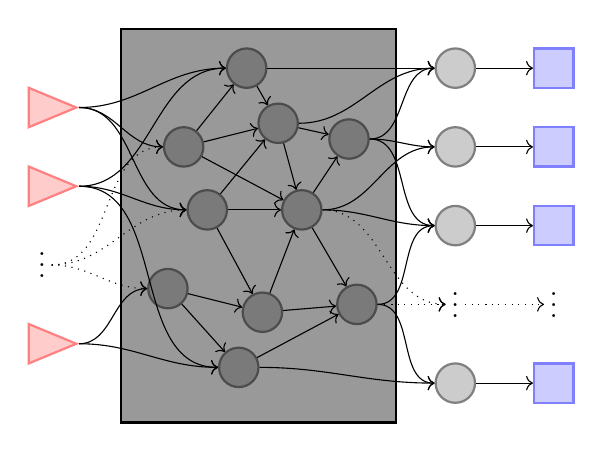
\begin{tikzpicture}
	[%
	input/.style ={isosceles triangle,	draw=red!50,		fill=red!20,		thick,	inner sep=0pt,	minimum size=5mm},%
	inner/.style ={circle,							draw=black!50,	fill=black!20,	thick,	inner sep=0pt,	minimum size=5mm},%
	output/.style={rectangle,					draw=blue!50,	fill=blue!20,	thick,	inner sep=0pt,	minimum size=5mm},%
	]

	\newcommand\lin{0}
	\newcommand\lhid{5.25}
	\newcommand{\lout}{6.5}
	
	% nodes
	\foreach \i in {0,2,3} \node (input\i) at (\lin,0.5+\i) [input] {};
	
	\foreach \i in {0,2,3,4} \node (output\i) at (\lout,\i) [output] {};
	
	\foreach \n/\x/\y in {	0/1.6/1.2, 1/1.8/3.0, 2/2.1/2.2, 3/2.5/0.2, 4/2.6/4.0, %
												5/2.8/0.9, 6/3.0/3.3, 7/3.3/2.2, 8/3.9/3.1, 9/4.0/1.0, %
												10/\lhid/0, 12/\lhid/2, 13/\lhid/3, 14/\lhid/4 %
												}
			\node (inner\n) at (\x,\y) [inner] {};
	
	\node (input1)		at (\lin,1.5) {}; 		\node at (\lin,1.6) {$\vdots$};
	\node (inner11)	at (\lhid,1.0) {}; 	\node at (\lhid,1.1) {$\vdots$};
	\node (output1)	at (\lout,1.0) {}; 	\node at (\lout,1.1) {$\vdots$};
	
	% interconnections
	% input to inner
	\foreach \i/\o in {0/0, 0/3, 2/2, 2/3, 2/4, 3/1, 3/2, 3/4}
		\draw [->] (input\i) to [out=0,in=180] (inner\o);
		
	\foreach \i/\o in {1/0, 1/1, 1/2}
		\draw [dotted, ->] (input\i) to [out=0,in=180] (inner\o);

	% inner to inner
	\foreach \i/\o in {	0/3, 0/5, 1/4, 1/6, 1/7, 2/5, 2/6, 2/7,%
											3/9, 4/6, 5/7, 5/9, 6/7, 6/8, 7/8, 7/9%
											}
		\draw [->] (inner\i) to (inner\o);
		
	\foreach \i/\o in {3/10, 9/10, 7/12, 8/12, 9/12, 7/13, 8/13, 4/14, 6/14, 8/14}
		\draw [->] (inner\i) to [out=0,in=180] (inner\o);
				
	\foreach \i/\o in {7/11, 9/11}
		\draw [dotted, ->] (inner\i) to [out=0,in=180] (inner\o);

	% inner to output
	\foreach \ii in {0, 2, 3, 4}
		\draw [->] (inner1\ii) to [out=0,in=180] (output\ii);
	\draw [dotted, ->] (inner11)  to [out=0,in=180] (output1);
	
	% black box
	\filldraw [thick, draw=black, fill=black, fill opacity=0.4] (1.0,-0.5) rectangle (4.5,4.5);
	
\end{tikzpicture}
	\caption{A reservoir NN is topologically equivalent to deep networks. However only the last layer is trained. In this picture the trained node are represented outside the box, while those inside are initialized with random weights which are then left unchanged.}
	\label{fig:reservoirNN}
\end{figure}

\noindent This kind of networks, then, can be trained much faster than their respective counterparts, i.e. feedforward and recurrent.
The question over which training method is more efficient is still debated and literature does not provide clear answers yet.

%\subsubsection{Modular NN}
%\label{sec:Modular_NN}

%\subsubsection{Spiking NN}
%\label{sec:Spiking_NN}
%Spiking artificial networks are the most different kind in respect to all the other networks until now described.
%In this class of ANNs, information is not coded only in the intensity of the signal, but also in the rate of signals, e.g. a high value will be encoded as a signal with high repetition rate, whereas a low value as a signal with low repetition rate.
%This way of encoding information is more alike the mechanism of biological neural networks, such as our brain \ref{}.
%
%\vspace{1em}
%\noindent LOOK INTO other type of neuron model: Hodgkin–Huxley (H-H) model\\
%\url{ https://en.wikipedia.org/wiki/Binding_neuron }

%\section{Real-Life Examples}
%\label{sec:Real-Life_Examples}
%\noindent\uppercase{\large{? Should I keep this section ?}}
%\normalsize

\section{ANN Simulation}
\label{sec:ANN_Simulation}
In the field of artificial neural network simulation, there are several platforms that are independently developed.
Among them there are TensorFlow, Theano, Caffe, Keras, Torch, and PyTorch.
Unfortunately, each one of them have its strength and weakness, therefore the choice of the framework becomes very difficult.

To make a choice, the key factors considered were the language used, the features, the flexibility, and the level of diffusion of the framework in the machine learning community.
The language used is a determining factor, because it takes time to learn the peculiarities of a library written for a known language, but even more time to learn to use an unknown programming language.
However also the features and the flexibility in the implementation are important traits, on account of the fact that any feature that is not natively implemented needs new coding.
In turn, it is difficult to integrate new coding if the framework is not flexible enough to accommodate extensions or custom definitions.
Last, but not least, it is easier to find support for a widespread framework in respect to a limitedly used one.
In regards to this, \autoref{fig:GoogleTrendsPyTorch} shows the number of internet searches for some frameworks in the past few years.

In light of the facts above, PyTorch was chosen as framework.
PyTorch is an open source machine learning library for python, which development has started only recently and it is based upon the older framework Torch  \cite{PyTorch.org}.
It provides a high-level platform for the deep learning ecosystem and integrates acceleration libraries that allow fast and lean operation, both on common \acsp{CPU} and \acsp{GPU}.
It is based on a backpropagation algorithm called \textit{Reverse-mode auto-differentiation}, which allows versatile execution.

To summarize, the library was chosen for its language, its flexibility, and the growing interest for it within the machine learning community.
Nevertheless, its features make it a very powerful framework. However, considering the need to keep the simulated system as simple as possible, this last characteristic slipped in the background.
The need to simulate a simple network comes from the fact that the ultimate goal of this project is to implement an \acs{ANN} with a (photonic) hardware architecture.

\begin{figure}[htbp]
	\centering
	\tikzsetexternalprefix{tikz/}	% set subfolder
\tikzsetnextfilename{GoogleTrendsPyTorch}

\begin{tikzpicture}[baseline]
	
	\begin{axis}[
			title={Google Trends Analytics},
			xlabel={Year},
			ylabel={Interest over time},
%			tick align=outside,
			width=\textwidth*0.75,%
			height=207pt,
			legend style={at={(0.5,-0.45)},anchor=north,legend columns=-1},
			date coordinates in=x,
			xtick distance={124},
			xticklabel={\month-\year},
			xticklabel style= {rotate=90,anchor=near xticklabel},
		]
			 
		\addplot [semithick, blue!80]
			table [x index=0, y index=1] {tikz/GTrends_multiTimeline.csv};
		\addplot [semithick, red]
			table [x index=0, y index=2] {tikz/GTrends_multiTimeline.csv};
		\addplot [semithick, orange]
			table [x index=0, y index=3] {tikz/GTrends_multiTimeline.csv};
		\addplot [semithick, green!60!blue]
			table [x index=0, y index=4] {tikz/GTrends_multiTimeline.csv};
		\addplot [semithick, black]
			table [x index=0, y index=5] {tikz/GTrends_multiTimeline.csv};
			
    \addlegendentry{ \scriptsize PyTorch }
    \addlegendentry{ \scriptsize TensorFlow }
    \addlegendentry{ \scriptsize Theano }
    \addlegendentry{ \scriptsize Keras }
    \addlegendentry{ \scriptsize Caffe }
    
	\end{axis}
\end{tikzpicture}
	\caption{Google Search statistics for different keywords in the \textit{machine learning and artificial intelligence} field.
		Numbers represent search interest relative to the highest point on the chart for the given region and time.
		A value of 100 is the peak popularity for the term.}
	\label{fig:GoogleTrendsPyTorch}
\end{figure}

%The resources and the time available allowed me to implement physically only the activation function of one node.
%Hence, to test this hardware implementation as I will show in \autoref{sec:Test_of_a_Trained ANN} of \autoref{ch:experiments}, I had first to simulate and train \textit{offline} a specific neural network.
%To do so, I chose a programming language, \textit{Python}, and a library, \textit{PyTorch}, which helped me in this task.

\subsection{PyTorch}
\label{ssec:PyTorch}
PyTorch is a Python package which provides a powerful framework for deep learning.
It is versatile in the sense that allow customizations at almost every level of operation.
For the purposes of this work, a neural network implemented in PyTorch is composed by the definition of three main components and a few lines of code to implement the operation.

The most important part of the network is the so called \textit{model}, which defines the topology of the network by setting parameters such as the number of nodes in each layer and the connections among them.
Moreover, it defines also the activation function for each node, separately or in groups.
The activation function can be coded from scratch, but can also be one of the functions provided by the library or a composition of them.
While the first offers almost unlimited flexibility, the second choice consents to exploit the functions already given.
The second option is the best choice, if the needs of the task support it, because it allows to save much time.

Another important part of the network is the so called \textit{criterion}, which is nothing else than the loss function.
The set of functions provided by PyTorch can accommodate almost any necessity.
Moreover, their operation can usually be adjusted with some internal parameters.

Similarly to the criterion, the last piece of the system is given by the \textit{optimizer}.
Optimizers are a class of algorithms that provides the optimization of the weights during the learning phase.
Most commonly used methods are already supported and they provide parameters to fine tune their execution.

Following the official tutorials and the immense package documentation, I implemented a fully connected \acf{MLP} model and then tested it with randomly generated numbers until its operation seemed correct.
The code that I implemented allows to change the overall structure of the network with some parameters (see \autoref{ssec:Simulated_ANN_operation})
The optimizer chosen is called \acfi{SGD}, which is parametrized just by the learning rate, at least in its vanilla implementation.
The criterion used initially was the mean square error, however it was eventually replaced by the \acfi{CEL}, which is more suited to the classification task.

\subsection{Dataset}
\label{ssec:PyDataset}
Initial tests and trials on artificial neural networks are often made by using randomly generated sets of numbers.
However, once the system has been successfully set up, to compare different working parameters such as number of nodes and number of layers, a common standardized dataset should be employed.
Moreover in this way, it is possible to compare implementations belonging to other research groups.

Again, the need to keep the system as simple as possible, drove my attention towards datasets of middle to small sizes.
With the help of the \textit{UC Irvine Machine Learning Repository} \cite{UCIMLR}, I selected one with a bit less than a thousand entries.
The dataset is called \textit{Connectionist Bench (Vowel Recognition - Deterding Data) Data Set}.
It is composed by \num{990} entries of \num{10} attributes, i.e. input values, grouped in \num{11} classes.

Each entry is a vector of \num{10} real numbers plus an integer number between \num{0} and \num{10}.
In view of the fact the proposed activation function is a real-positive-valued function (see \autoref{sec:Characterization_of_the_Activation_Function}), I renormalized the database.
The normalization is independently applied to each one of the attributes in such a way that is described by a real number in $[0,1]$.
The normalization is applied before the dataset is divided in the learning and testing examples.

The authors suggest to divide the dataset a learning set of \num{528} entries and a testing set of \num{462} entries.
Since the number of entries is low, compared to other datasets, the validation set is not define.
In this case, the test set is used as validation instead too.

\subsection{Simulated ANN operation}
\label{ssec:Simulated_ANN_operation}
The model that I defined allows some changes with the simple definition of a few parameters.
Specifically, the parameters cover the number of input and ouptut nodes, the number of hidden layer, and the number of nodes in each hidden layer.
Whereas the number of input and output nodes is defined by the problem, i.e. the dataset, the other are free parameters that can
Another degree of freedom that I implemented is whether the last hidden layer applies the nonlinear activation function or just the weighted sum, since I observed that many network in the tutorials were built this way.
The scheme of the network is shown in \autoref{fig:ANN_model}.

\begin{figure}[htbp]
	\centering
	\tikzsetnextfilename{PT_MLP}%	
%	% nodes
%	\foreach \i in {0,1,3} \node (input\i) at (\lin,2.5-\i) [input] {};
	
%	\foreach \j in {\lhid,\lhidb,\lhidd}
%		\foreach \i in {0,1,2,4} \node (inner\j_\i) at (\j,3-\i) [inner] {};
%	\foreach \j in {\lhide}%
%	\foreach \i in {0,1,3} \node (inner\lhide_\i) at (\lhide,2.5-\i) [inner] {};
%	
%	\foreach \i in {0,1,3} \node (output\i) at (\lout,2.5-\i) [output] {};
%	
%	\node (input2)		at (\lin,0.5) {}; 		\node at (\lin,0.6) {$\vdots$};
%	\foreach \j in {\lhid,\lhidb,\lhidd}%
%		\node (inner\j_3)		at (\j,0.0) {};
%	\foreach \j in {\lhid,\lhidb,\lhidd}%
%		\node at (\j,0.1) {$\vdots$};
%	\node (inner\lhide_2) at (\lhide,0.5){}; \node at (\lhide,0.6) {$\vdots$};
%	\node (output2)	at (\lout,0.5) {}; 	\node at (\lout,0.6) {$\vdots$};
	
	% interconnections
	% in - hid1
%	\foreach \i in {0,1,3}%
%		\foreach \j in {0,1,2,4}%
%			\draw [->] (input\i) to [out=0, in=180] (inner\lhid_\j);
%	\foreach \i in {0,1,3}%
%		\draw [dotted, ->] (input\i)	to [out=0, in=180] (inner\lhid_3);
%	\foreach \j in {0,1,2,4}%
%		\draw [dotted, ->] (input2) 	to [out=0, in=180] (inner\lhid_\j);
%	
%	\foreach \i in {0,1,2,4}%
%		\foreach \j in {0,1,2,4}%
%			\draw [->] (inner\lhid_\i) to [out=0, in=180] (inner\lhidb_\j);
%	\foreach \i in {0,1,2,4}%
%		\draw [dotted, ->] (inner\lhid_\i)	to [out=0, in=180] (inner\lhidb_3);
%	\foreach \j in {0,1,2,4}%
%		\draw [dotted, ->] (inner\lhid_3) to [out=0, in=180] (inner\lhidb_\j);
%	
%	\foreach \i in {0,1,2,3,4}%
%		\foreach \j in {0,1,2,3,4}%
%			\draw [dotted,->] (inner\lhidb_\i) to [out=0, in=180] (inner\lhidd_\j);
%	\fill [white] (6.3,-1.5) rectangle (6.7,3.5);
%	\foreach \i in {-0.9,0.1,1.1,2.1,3.1}%
%		\node at (\lhidc,\i) {$\vdots$};
%
%%	\foreach \i in {0,1,3}%
%%		\draw [->] (inner\lhidd_\i) to [out=0, in=180] (output\i);
%	\foreach \i in {0,1,3}%
%		\draw [->] (inner\lhide_\i) to [out=0, in=180] (output\i);
%
%	\draw [dotted, ->] (inner\lhide_2) to [out=0, in=180] (output2);
	
%\end{tikzpicture}

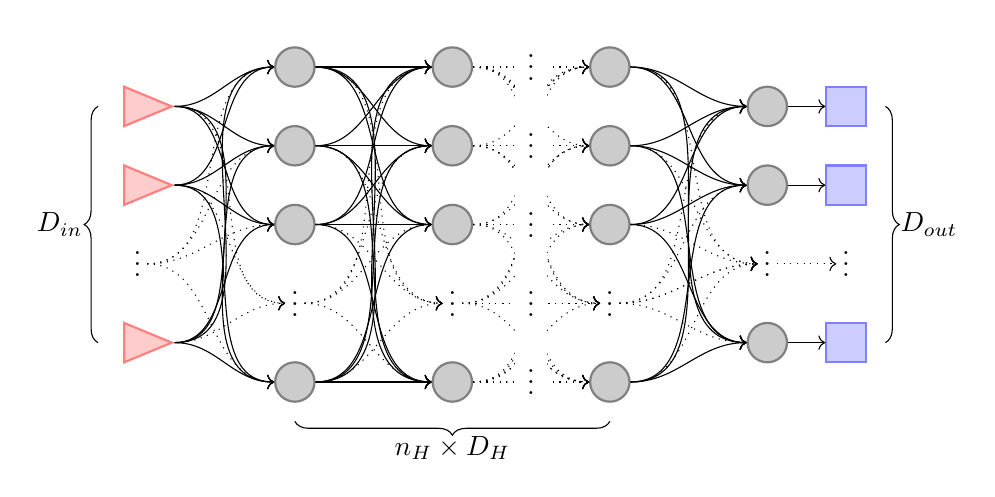
\begin{tikzpicture}
	[%
	input/.style ={isosceles triangle,	draw=red!50,		fill=red!20,		thick,	inner sep=0pt,	minimum size=5mm},%
	inner/.style ={circle,							draw=black!50,	fill=black!20,	thick,	inner sep=0pt,	minimum size=5mm},%
	output/.style={rectangle,					draw=blue!50,	fill=blue!20,	thick,	inner sep=0pt,	minimum size=5mm},%
	]

	\newcommand{\lin}{0}
	\newcommand{\lhid}{2}
	\newcommand{\lhidb}{4}
	\newcommand{\lhidc}{5}
	\newcommand{\lhidd}{6}
	\newcommand{\lhide}{8}
	\newcommand{\lout}{9}
	
	% nodes
	\foreach \i in {0,1,3} \node (input\i) at (\lin,2.5-\i) [input] {};
	
	\foreach \j in {\lhid,\lhidb,\lhidd}%
		\foreach \i in {0,1,2,4} \node (inner\j_\i) at (\j,3-\i) [inner] {};
	\foreach \i in {0,1,3} \node (inner\lhide_\i) at (\lhide,2.5-\i) [inner] {};
	\foreach \i in {0,1,3} \node (output\i) at (\lout,2.5-\i) [output] {};
	
	\node (input2)		at (\lin,0.5) {}; 		\node at (\lin,0.6) {$\vdots$};
	\foreach \j in {\lhid,\lhidb,\lhidd}%
		\node (inner\j_3)		at (\j,0.0) {};
	\foreach \j in {\lhid,\lhidb,\lhidd}%
		\node at (\j,0.1) {$\vdots$};
	\node (inner\lhide_2) at (\lhide,0.5){}; \node at (\lhide,0.6) {$\vdots$};
	\node (output2)	at (\lout,0.5) {}; 	\node at (\lout,0.6) {$\vdots$};
	
	% interconnections
	% in - hid1
	\foreach \i in {0,1,3}%
		\foreach \j in {0,1,2,4}%
			\draw [->] (input\i) to [out=0, in=180] (inner\lhid_\j);
	\foreach \i in {0,1,3}%
		\draw [dotted, ->] (input\i)	to [out=0, in=180] (inner\lhid_3);
	\foreach \j in {0,1,2,4}%
		\draw [dotted, ->] (input2) 	to [out=0, in=180] (inner\lhid_\j);
	
	\foreach \i in {0,1,2,4}%
		\foreach \j in {0,1,2,4}%
			\draw [->] (inner\lhid_\i) to [out=0, in=180] (inner\lhidb_\j);
	\foreach \i in {0,1,2,4}%
		\draw [dotted, ->] (inner\lhid_\i)	to [out=0, in=180] (inner\lhidb_3);
	\foreach \j in {0,1,2,4}%
		\draw [dotted, ->] (inner\lhid_3) to [out=0, in=180] (inner\lhidb_\j);
	
	\foreach \i in {0,1,2,3,4}%
		\foreach \j in {0,1,2,3,4}%
			\draw [dotted,->] (inner\lhidb_\i) to [out=0, in=180] (inner\lhidd_\j);
	\fill [white] (4.8,-1.5) rectangle (5.2,3.5);
	\foreach \i in {-0.9,0.1,1.1,2.1,3.1}%
		\node at (\lhidc,\i) {$\vdots$};
	\foreach \i in {0,1,2,3,4}%
		\draw [dotted, ->] (inner\lhidd_\i)	to [out=0, in=180] (inner\lhide_2);
	\foreach \j in {0,1,2,3}%
		\draw [dotted, ->] (inner\lhidd_3) to [out=0, in=180] (inner\lhide_\j);

	\foreach \i in {0,1,2,4}%
		\foreach \j in {0,1,3}
			\draw [->] (inner\lhidd_\i) to [out=0, in=180] (inner\lhide_\j);
	\foreach \i in {0,1,3}
			\draw [->] (inner\lhide_\i) to [out=0, in=180] (output\i);

	\draw [dotted, ->] (inner\lhide_2) to [out=0, in=180] (output2);
	
	\draw [decorate, decoration={brace, amplitude=5}] (\lhidd,-1.5) -- (\lhid,-1.5)
		node [midway, below=2pt] {$n_{H}\times D_H$};
	\draw [decorate, decoration={brace, amplitude=5}] (-.5,-0.5) -- (-.5,2.5)
		node [midway, left=2pt]  {$D_{in}$};
	\draw [decorate, decoration={brace, amplitude=5}] (9.5,2.5) -- (9.5,-0.5)
		node [midway, right=2pt] {$D_{out}$};
	
\end{tikzpicture}
	\caption{Topology of the model implemented in PyTorch. The number of input ($D_{in}$) ad output nodes ($D_{out}$), as well as the number of nodes in the last hidden layer is determined by the dataset.
	The number of nodes ($D_{H}$) in the other hidden layers and the number of hidden layers itself ($n_{H}$) is governed by a parameter.}
	\label{fig:ANN_model}
\end{figure}

The choice of the structure of the neural network is purely heuristic, since up to now no satisfactory method has been proposed in literature.
However, given the problem (dataset), at least the input and output layer have a fixed amount of nodes.
Specifically, the input nodes are \num{10}, the number of attributes, while the output nodes are \num{11}, the number of classes.

Using the chosen dataset, I tested the neural network operation on the model defined before, with two different kinds of activation function.
Initially I implemented a \acfi{ReLU} and a \textit{Logistic} (sigmoid) activation functions.
The \acs{ReLU} function is a standard activation function and is defined as follows:
\begin{equation}
f_{ReLU}(x) =
\begin{cases}
	0 & \qquad \mathrm{for}~ x\leq 0\\
	x & \qquad \mathrm{for}~ x\geq 0
\end{cases}~.
\label{eq:relu}
\end{equation}
On the other hand, the Logistic function, which has already been shown in \autoref{fig:activation_function_example_2}, is defined by
\begin{equation}
f_{Logistic}(x) = \frac{1}{1+e^{-k\left(x-x_0\right)}},
\end{equation}
with the parameters $k\in \mathcal{R}^+$ and $x_0\in \mathcal{R}$.
Both functions are widely used in literature, however the \acs{ReLU} function seems to be preferred lately.
I will discuss in \autoref{sec:Test_of_a_Trained ANN} the results of the same network models, with the nonlinear activation function given by the microring resonator.

\subsubsection{Learning}
After the definition of the model, I had to train the networks on the training set.
Since the dataset is small, all the examples are fed into the model, then the overall loss is evaluated, and finally the weights are upgraded.
This method is called \textit{batch} operation; others are \textit{online} operation, which evaluate the loss and change the weights at each example, and \textit{minibatch} operation, which uses a random subset of the full dataset.

Every time the network is trained on the full dataset, an \textit{epoch} is completed.
I trained the models defined above for \num{2000} epochs, in order to observe both the fast and slow dynamics.
For example, smaller networks tend to train faster, because there are less free parameters.
On the other hand, larger networks often train slower, but can obtain better results thanks to their complexity.

Moreover, I defined a different learning rates $l_r$ for each activation function, in order to provide the best parameter for different models but still be able to compare the performance of similar ones.
Specifically the learning rate for the \acs{ReLU} is $l_{r|ReLU} = \num{5e-2}$, while for the Logistic function is $l_{r|Logistic}= \num{5e-3}$

\begin{figure}[htbp]
	\centering
	\tikzsetexternalprefix{tikz/}	% set subfolder
\tikzsetnextfilename{Train_evolution}

%\newcommand{\righttriangles}[1]{
%    \pgfplotstableread[col sep=tab, header=true]{#1}{\table}
%    \pgfplotstablegetcolsof{#1}
%    \pgfmathtruncatemacro\numberofcols{\pgfplotsretval - 1}
%    \pgfplotsinvokeforeach{1,...,\numberofcols}{
%        \pgfplotstablegetcolumnnamebyindex{##1}\of{\table}\to{\colname}
%        \addplot [name path=down##1, semithick, color##1, mark=*, mark size=1, mark options={solid}]%
%        		table [x index= 0, y index=##1] {#1};
%        \addlegendentryexpanded{ \SI{\colname}{\mW} }
%    }
%}

%\newcommand{\lefttriangles}[1]{
%    \pgfplotstableread[col sep=tab, header=true]{#1}{\table}
%    \pgfplotstablegetcolsof{#1}
%    \pgfmathtruncatemacro\numberofcols{\pgfplotsretval - 1}
%    \pgfplotsinvokeforeach{1,...,\numberofcols}{
%        \pgfplotstablegetcolumnnamebyindex{##1}\of{\table}\to{\colname}
%        \addplot [name path=up##1, semithick, color##1, mark=*, mark size=1, mark options={solid}]%
%        		table [x index= 0, y index=##1] {#1};
%    }
%}

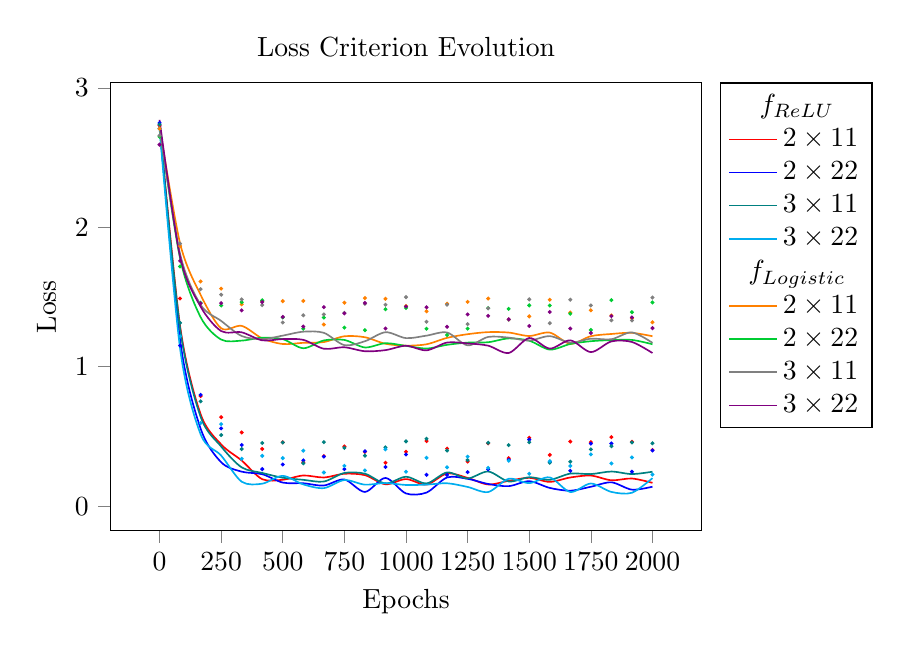
\begin{tikzpicture}[baseline]

%	\definecolor{color1}{rgb}{0.12156862745098,0.466666666666667,0.705882352941177}
%	\definecolor{color2}{rgb}{1,0.498039215686275,0.0549019607843137}
%	\definecolor{color3}{rgb}{0.172549019607843,0.627450980392157,0.172549019607843}
%	\definecolor{color4}{rgb}{0.83921568627451,0.152941176470588,0.156862745098039}
%	\definecolor{color5}{rgb}{0.580392156862745,0.403921568627451,0.741176470588235}
%	\definecolor{color6}{rgb}{0.549019607843137,0.337254901960784,0.294117647058824}
%	\definecolor{color7}{rgb}{0.890196078431372,0.466666666666667,0.76078431372549}
%	\definecolor{color8}{rgb}{0.45,0.45,0.45}
%	\definecolor{color9}{rgb}{0.25,0.25,0.99}
	
	\begin{axis}[
			title={Loss Criterion Evolution},
			xlabel={Epochs},
			ylabel={Loss},
			tick align=outside,
			tick pos=left,
			width=\textwidth*0.75,
			height=207pt,
			legend pos = outer north east,
%			cycle list name=color list,
			/pgf/number format/1000 sep=,
%			xmin=-199, xmax=2199,
			xtick distance=250,
			domain=0:2000,
			train/.style={
				smooth,
				semithick,
			},
			valid/.style={
				only marks,
				mark=*,
				mark options={scale=0.25},
				forget plot,
			},
		]
		\addlegendentry{\hspace{-.6cm}$f_{ReLU}$};
		\addlegendimage{empty legend};

		\addplot [red, train] {0.2+2.5*exp(-0.01*x)+0.05*rand};
		\addlegendentry{$2\times 11$}
		\addplot [red, valid] {0.4+2.3*exp(-0.01*x)+0.1*rand};
		
		\addplot [blue, train] {0.15+2.6*exp(-0.011*x)+0.06*rand};
		\addlegendentry{$2\times 22$}
		\addplot [blue, valid] {0.35+2.35*exp(-0.012*x)+0.13*rand};

		\addplot [teal, train] {0.2+2.5*exp(-0.01*x)+0.05*rand};
		\addlegendentry{$3\times 11$}
		\addplot [teal, valid] {0.4+2.3*exp(-0.01*x)+0.1*rand};
		
		\addplot [cyan, train] {0.15+2.6*exp(-0.011*x)+0.06*rand};
		\addlegendentry{$3\times 22$}
		\addplot [cyan, valid] {0.35+2.35*exp(-0.012*x)+0.13*rand};
%		red,blue,black,yellow,brown,teal,orange,violet,cyan,green!70!black,magenta,gray
		
		\addlegendentry{\hspace{-.6cm}$f_{Logistic}$}
		\addlegendimage{empty legend};
		
		\addplot [orange, train] {1.2+1.5*exp(-0.01*x)+0.05*rand};
		\addlegendentry{$2\times 11$}
		\addplot [orange, valid] {1.4+1.3*exp(-0.01*x)+0.1*rand};
		
		\addplot [blue!20!green, train] {1.15+1.6*exp(-0.011*x)+0.06*rand};
		\addlegendentry{$2\times 22$}
		\addplot [blue!20!green, valid] {1.35+1.35*exp(-0.012*x)+0.13*rand};	
		
		\addplot [gray, train] {1.2+1.5*exp(-0.01*x)+0.05*rand};
		\addlegendentry{$3\times 11$}
		\addplot [gray, valid] {1.4+1.3*exp(-0.01*x)+0.1*rand};
		
		\addplot [violet, train] {1.15+1.6*exp(-0.011*x)+0.06*rand};
		\addlegendentry{$3\times 22$}
		\addplot [violet, valid] {1.35+1.35*exp(-0.012*x)+0.13*rand};
		
	\end{axis}
\end{tikzpicture}
	\caption{Evolution of the loss criterion (solid lines) throughout the epochs.
		Points represent the values of the loss criterion on the validation dataset, carried out repeatedly during the training.
	}
	\label{fig:PyTorch_learning}
\end{figure}

\autoref{fig:PyTorch_learning} shows the evolution of the loss and the validation of each model during the \num{2000} epochs of training.
From the evolution of the loss function we can see that every model has 


\subsubsection{Collection of results}
Since the number of classes is \num{11}, the percentage of correct answer given a random value is $\sim \SI{9.09}{\percent}$.
Hence, values of correct answers above that mean that the neural network is working.
On the other hand, values around or even below \SI{9.09}{\percent} mean that the current neural network is not working at all.

\autoref{tab:PyResults} collects all the results for the different topologies.
The same shape has been tested with both $f_{ReLU}$ and $f_{Logistic}$ to compare the performance.

\begin{table}[htbp]
	\centering
	\begin{tabular}{c c c c r}
	\toprule
	activation	& no. hidden 	& no. nodes	& other			& Percent\\
	function		& layers 			& per layer	& parameters	& correct\\
	\midrule
	$f_{ReLU}$ 			& 2 & 11 & - & \SI{70}{\percent}\\
	$f_{ReLU}$ 			& 2 & 22 & - & \SI{70}{\percent}\\
	$f_{ReLU}$ 			& 3 & 11 & - & \SI{70}{\percent}\\
	$f_{ReLU}$ 			& 3 & 22 & - & \SI{70}{\percent}\\
	$f_{Logistic}$ 	& 2 & 11 & - & \SI{9}{\percent}\\
	$f_{Logistic}$ 	& 2 & 22 & - & \SI{9}{\percent}\\
	$f_{Logistic}$ 	& 3 & 11 & - & \SI{9}{\percent}\\
	$f_{Logistic}$ 	& 3 & 22 & - & \SI{9}{\percent}\\
	\bottomrule
	\end{tabular}
	\caption{Results of the different activation functions and the several network topologies.
	}
	\label{tab:PyResults}
\end{table}

%+-------------------------+--------+---------+---------+
%|                         | no. of | no.     | percent |
%|       Classifier        | hidden | correct | correct |
%|                         | units  |         |         | 
%+-------------------------+--------+---------+---------+
%| Single-layer perceptron |  -     | 154     | 33      | 
%| Multi-layer perceptron  | 88     | 234     | 51      |
%| Multi-layer perceptron  | 22     | 206     | 45      |
%| Multi-layer perceptron  | 11     | 203     | 44      | 
%| Modified Kanerva Model  | 528    | 231     | 50      |
%| Modified Kanerva Model  | 88     | 197     | 43      | 
%| Radial Basis Function   | 528    | 247     | 53      |
%| Radial Basis Function   | 88     | 220     | 48      | 
%| Gaussian node network   | 528    | 252     | 55      |
%| Gaussian node network   | 88     | 247     | 53      |
%| Gaussian node network   | 22     | 250     | 54      |
%| Gaussian node network   | 11     | 211     | 47      | 
%| Square node network     | 88     | 253     | 55      |
%| Square node network     | 22     | 236     | 51      |
%| Square node network     | 11     | 217     | 50      | 
%| Nearest neighbour       |  -     | 260     | 56      | 
%+-------------------------+--------+---------+---------+

% second chapter "Photonics applied to ANNs" ~ 15pg
\chapter{Photonics applied to ANNs}

How do I intend to create a hardware photonic ANN node?
\section{Weighted sum of inputs}
This has already been demonstrated and integrated widely, so it will not be the focus of this work.
\section{Nonlinear activation function}
On the other hand, a photonic nonlinear activation function has not yet been found.
This is where the focus of my work will be.

\subsection{Simulations}

% third chapter "Samples, setup and measurements" ~ 20pg
\chapter{Samples, setup and experiments}
\label{ch:experiments}

All the experiments have been carried out on \acs{PIC} developed within a FP7 project (IRIS, \cite{testa2016design}) that aimed to develop an optical router.
An optical router is a matrix of microresonators whose resonances are tuned at will to (re)direct an optical signal along a predefined path.
We exploit the nonlinear optical response of these nodes to demonstrate the feasibility of an all optical nonlinear activation function made on PIC.

%All the experiments have been carried out on samples manufactured for the IRIS project \cite{testa2016design}.
%This is due to the fact that in the time frame of this work there would have not been enough time to design and produce an ad hoc device.
%Moreover, as already stated, the aim of this thesis is to produce a proof of concept for an all-optical implementation of an activation function, rather than to construct a complete prototype.
%With the knowledge obtained during this work, future researches could design new structures by focusing on the correct parameters.

\section{The samples}
The IRIS project studied the design and the implementation of an integrated reconfigurable silicon photonics switch matrix, a routing device, as a replacement for electronic devices used in the telecommunication industry.
The completed integrated photonic circuit consists of a matrix of waveguides crossing each other and linked by couples of racetrack resonators, thermally-controlled.
At the ends of the waveguides other structures, interleavers and \acsp{AWG}, allowed many signals at different wavelengths to be multiplexed/demultiplexed onto/from the same waveguide.

\begin{figure}[hbtp]
	\centering
	\tikzsetexternalprefix{tikz/}	% set subfolder
\tikzsetnextfilename{IRIS}
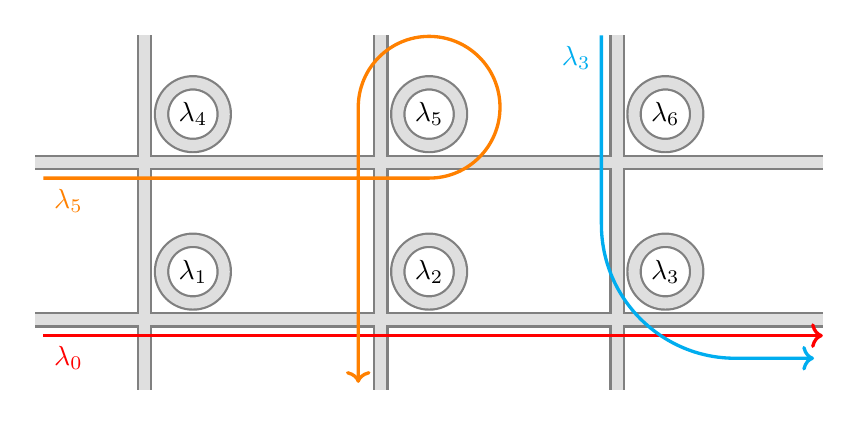
\begin{tikzpicture}[
		baseline,
		wave/.style	={ 
			very thick, line cap=butt, ->,
			%rounded corners=128pt,
		},
		guide/.style 	={ double=gray!25, double distance=4pt,
			thick, draw=black!50,
			rounded corners=4pt, line join=round, line cap=butt,
		},
		ring/.style 		={ circle, radius=64pt,
			double=gray!25, double distance=4pt,
			thick, draw=black!50,
			rounded corners=8pt, line join=round,
		},
	]
	
	\def\mylist{ 0/0/1, 3/0/2, 6/0/3, 0/2/4, 3/2/5, 6/2/6}
	
	% draw rings
	\foreach \x/\y/\n in \mylist
		\node [ring] (ring_\n) at (\x,\y) {$\lambda_\n$};
	
	% draw waveguides
	\draw [guide]
			% insert the horizontal wgs here
			(ring_1.south)++(-2,-0.2) -- ++(10,0)
			(ring_4.south)++(-2,-0.2) -- ++(10,0)
			% insert the vertical wgs here
			(ring_1.west)++(-0.2,-1.5) -- ++(0,4.5)
			(ring_2.west)++(-0.2,-1.5) -- ++(0,4.5)
			(ring_3.west)++(-0.2,-1.5) -- ++(0,4.5);
			
	% draw waves
	\draw [wave, red] (ring_1.south)++(-1.9,-0.4) node [below right] {$\lambda_0$} -- ++(9.9,0);
	\draw [wave, orange] (ring_4.south)++(-1.9,-0.4) node [below right] {$\lambda_5$} -- ++(4.9,0)
				arc (-90:180:0.9) -- ++(0,-3.5);
	\draw [wave, cyan] (ring_6.west)++(-0.4, 1) node [below left] {$\lambda_3$} -- ++(0,-2.4)
				arc (180:270:1.7) -- ++(1,0);
	
\end{tikzpicture}

	\caption{Scheme of a routing node of the full \acs{PIC} of IRIS. $\lambda_0$ travels from the input port to the through port; $\lambda_5$ is redirected from the input port to the drop port; $\lambda_3$ is redirected from an add port to the through port.}
	\label{fig:fullmatrix}
\end{figure}

Each node of the matrix can be modeled by a microring resonator in \acs{ADF} configuration (see \autoref{ssec:Microring_optical_cavity}).
Any signal that enters a node detuned from the resonance of the microring is directed toward the through port of the node.
On the other hand, any signal that enters a node in resonance with the microring is redirected toward the drop port.
\autoref{fig:fullmatrix} shows the scheme of a node in the full \acs{PIC}, where the signals is routed.

%The complexity of such photonic circuit required outstanding precision in the design and the fabrication.
%Hence, for preliminary testing purposes, each and every structure of which the full device is composed, has been manufactured repeatedly with several small variations.
%For example, several microrings in the \ac{ADF} configuration have been fabricated with different radius, or different ring-waveguide gap.
%The collection of all these testing structures on the same chip was produced in a few samples.
%All these test structures as well as a fully completed switch matrix were disposed on a single chip, accessible via grating couplers.

\newpage
The development of the final IRIS chip has required several steps of improvement and few generation of test samples were fabricated with different optical properties.
Thus the first step of the thesis has been to choose, among the many different devices available, the most promising ones.
%characterize qualitatively the response of some devices among the single structures, the short sequences of structures, and the full switch matrix itself.
%After many trials of different devices, my final choice was to study a system of intermediate complexity.
%In fact, since the work in this thesis is like the first step in a long journey, with this choice I tried to obtain a compromise between simplicity in immediate future (current work) and adaptability in the long term.
%For example, the current structure allowed me to study the nonlinear activation function, but could be reused in the future to study the weighted sum.
The structure selected (nicknamed \textit{mini-matrix}) is shown in \autoref{fig:photos} and it is composed by: a waveguide, coupled to eight drop channels through ring resonators.
In this family of devices, there were mini-matrices built with single microrings, double microrings, single racetracks, or double racetracks.
%The final choice was to study the \textit{mini-matrix} in which the coupling mechanism was provided by single ring resonators, because of its simpler transfer function in respect to double microrings or double racetracks.
\autoref{fig:minimatrix_scheme} shows a simplified scheme of the \textit{mini-matrix}.

\begin{figure}[htbp]
	\centering
	\begin{subfigure}[b]{0.7\textwidth}
		\centering
		\includegraphics[width=\textwidth]{photos/minimatrix.png}
		\caption{mini-matrix}
		\label{fig:photo_minimatrix}
	\end{subfigure}
	\begin{subfigure}[t]{0.345\textwidth}
		\centering
		\includegraphics[width=\textwidth]{photos/ring.png}
		\caption{microring}
		\label{fig:photo_ring}
	\end{subfigure}
	\begin{subfigure}[t]{0.345\textwidth}
		\centering
		\includegraphics[width=\textwidth]{photos/grating.png}
		\caption{grating}
		\label{fig:photo_grating}
	\end{subfigure}
	\caption{Magnified photograph of the \textit{mini-matrix} device chosen (a) and two important structures: (b) microring resonator and (c) output grating couplers. }
	\label{fig:photos}
\end{figure}

\begin{figure}[hbtp]
	\centering
%	\includegraphics[scale=.4]{figures/miniMATRIX_Klayout.png}\\
	\tikzsetexternalprefix{tikz/}	% set subfolder
\tikzsetnextfilename{miniMATRIX_scheme}
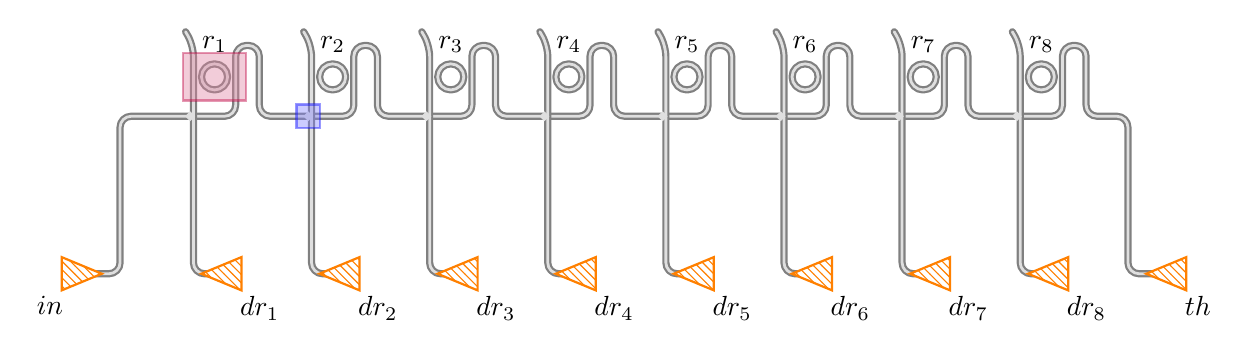
\begin{tikzpicture}[
		baseline,
		grating/.style	={ isosceles triangle, rotate=180,
			draw=orange, preaction={fill, white},
			pattern color=orange, pattern=north west lines,
			thick,
			inner sep=0pt,	minimum size=12pt
		},
		guide/.style 	={ double=gray!25, double distance=1pt,
			thick, draw=black!50,
			rounded corners=4pt, line join=round, line cap=round,
		},
		ring/.style 		={ circle, radius=16pt,
			double=gray!25, double distance=1pt,
			thick, draw=black!50,
			rounded corners=8pt, line join=round,
		},
	]
	
	\def\mylist{	1/0.0/0, 2/1.5/0, 3/3.0/0, 4/4.5/0,
									5/6.0/0, 6/7.5/0, 7/9.0/0, 8/10.5/0}

	% declare node of gratings and coupling regions
	\node (input) at (-2,0) {};
	\foreach \name/\px/\py in \mylist {
			\draw (\px,\py) node (dr\name) {} ++(-0.2,2.5) node (cr\name) {};
		}
	\draw (12.0,0) node (th) {};

	% draw rings
	\foreach \name/\px/\py in \mylist {
			\node (r\name) [ring] at (cr\name) {};
			\node at (r\name.north) [above] {$r_\name$};
			\draw (cr\name.west) ++(-0.02,0) node (rL\name) {};
			\draw (cr\name.east) ++(+0.02,0) node (rR\name) {};
		}
		
	% draw waveguides
	\draw [guide] (input) to (-1.4,0) -- (-1.4,2)
			% insert all the bendings here
			-| (rR1.east) -- ++(0,.4) -- ++(.3,0) -- ++(0,-0.9)
			-| (rR2.east) -- ++(0,.4) -- ++(.3,0) -- ++(0,-0.9)
			-| (rR3.east) -- ++(0,.4) -- ++(.3,0) -- ++(0,-0.9)
			-| (rR4.east) -- ++(0,.4) -- ++(.3,0) -- ++(0,-0.9)
			-| (rR5.east) -- ++(0,.4) -- ++(.3,0) -- ++(0,-0.9)
			-| (rR6.east) -- ++(0,.4) -- ++(.3,0) -- ++(0,-0.9)
			-| (rR7.east) -- ++(0,.4) -- ++(.3,0) -- ++(0,-0.9)
			-| (rR8.east) -- ++(0,.4) -- ++(.3,0) -- ++(0,-0.9)
			-- (11.4,2) -- (11.4,0) -- (th);

	\foreach \name/\px/\py in \mylist {
			\draw [guide] (dr\name) -| (rL\name.west) -- ++(0,0.4)  -- ++(120:0.2);
		}
	\foreach \px in {-.51,.99,2.49,3.99,5.49,6.99,8.49,9.99}
		\node [shape=diamond, draw=gray!25, fill=gray!25, inner sep=.8pt] at (\px,2) {};
	
	% draw gratings
	\node (grin) at (input) [grating, rotate=180] {};
	\node at (grin.south) [below left] {$in$};
	\foreach \name/\px/\py in \mylist{
			\node (gr\name) [grating] at (dr\name) {};
			\node at (gr\name.north) [below right] {$dr_\name$};
		}
	\node (grth) at (th) [grating] {};
	\node at (grth.north) [below right] {$th$};

	% draw highlighted areas
	\draw [thick, draw=purple, fill=purple!50, opacity=0.4] (r1)
				++(-0.4,-0.3) rectangle ++(0.8,0.6);
	\draw [thick, draw=blue, fill=blue!50, opacity=0.4]
				(.84,1.85) rectangle ++(0.3,0.3);
	
\end{tikzpicture}
	\caption{
		Simplified scheme of the \textit{mini-matrix} integrated photonic circuit (structures are not in scale).
		Triangles (orange) are the grating couplers ($in$, $dr_{1-8}$, $th$).
		Waveguides and rings ($r_{1-8}$) are shown as thick grey lines.
		The bigger (purple) highlighted area is a coupling region, shown in \autoref{fig:minimatrix_scheme_zoom}.
	}
	\label{fig:minimatrix_scheme}
\end{figure}

The resonance of each microring is strictly defined by the design of the structure, however it is ultimately changed by imperfections and uncertainties of the manufacturing process.
Hence, since the optical router requires precise positioning of the resonances, their fine tuning is obtained by controlling the temperature of the material.
Each one of the microring resonators in the structure has been manufactured with a thermo-electric heater, which is used to produce the thermo-optic effect (see \autoref{ssec:Thermal_nonlinearities}) in order to induce the required resonance tuning \cite{testa2016design}.
\autoref{fig:minimatrix_scheme_zoom} shows the scheme of the microring resonator geometry, without any non-optical structures (e.g. heaters, metallic contacts).
%This feature has never been exploited in this work, but could come of use in the future.

\begin{figure}[htbp]
	\centering
%	\includegraphics[scale=.4]{figures/single_ring_zoom.png}\\
	\tikzsetexternalprefix{tikz/}	% set subfolder
\tikzsetnextfilename{miniMATRIX_scheme_zoom}
\begin{tikzpicture}[
		baseline,
		scale=0.6,
		every pin edge/.style={-},
	]

%	\draw [help lines] (-3,-3) grid (3,3);
	
	\filldraw [draw=black!50, fill=gray!20, even odd rule]
		(0,0) circle [radius=4.43, thick]
		(0,0) circle [radius=4.91, thick];
	\path [name path=inner] (0,0) circle [radius=5.085];
	\path [name path=outer] (0,0) circle [radius=5.505];
	%distance between waveguides is 9.848
	\path [name path=leftwg]  (-4.924,-6) rectangle (-5.344,+6);
	\path [name path=rightwg] (+4.924,-6) rectangle (+5.344,+6);
	
	\path [name intersections={of=inner and leftwg, name=leftyin}];
	\path [name intersections={of=outer and leftwg, name=leftyout}];
	
	\path [name intersections={of=inner and rightwg, name=rightyin}];
	\path [name intersections={of=outer and rightwg, name=rightyout}];
	
	\draw [black!50, line join=round, rounded corners=1pt, fill=gray!20]
		(-4.924,-6) -- (-5.344,-6) -- (leftyout-4)
		.. controls ++(+103:1) and ++(-103:1) .. (leftyout-2)
		-- (-5.344,+6) -- (-4.924,+6) -- (leftyin-1)
		.. controls ++(-102:1) and ++(+102:1) .. (leftyin-2)
		-- cycle;
	
	\draw [black!50, line join=round, rounded corners=1pt, fill=gray!20]
		(+4.924,-6) -- (+5.344,-6) -- (rightyout-4)
		.. controls ++(+77:1) and ++(-77:1) .. (rightyout-2)
		-- (+5.344,+6) -- (+4.924,+6) -- (rightyin-1)
		.. controls ++(-78:1) and ++(+78:1) .. (rightyin-2)
		-- cycle;
	
	\draw [-stealth] (0,0) -- ++(60:4.43) node [left, midway] {$R_{in}$};
				
	\draw [|-|,black, thick] (+4.430,+0) -- (+4.910,+0) node [pin=+60:\SI{0.48}{\um}] {};
	\draw [|-|,black, thick] (+4.924,-3) -- (+5.344,-3) node [pin=+60:\SI{0.42}{\um}] {};
	\draw [|-|,black, thick] (-4.924,+0) -- (-5.085,+0) node [pin=120:\SI{0.175}{\um}] {};
	
	\draw [thick, -stealth] (+6.0,-6) -- (+6.0,-5) node [midway, right] {in};
	\draw [thick, -stealth] (+6.0,+5) -- (+6.0,+6) node [midway, right] {through};
	\draw [thick, -stealth] (-6.0,-5) -- (-6.0,-6) node [midway, left] {drop};
	\draw [thick, -stealth] (-6.0,+6) -- (-6.0,+5) node [midway, left] {add};

\end{tikzpicture}
	\caption{
	Microring optical cavity region, structures are in scale.
	The ring has an internal radius of $R_{in}=\SI{4.43}{\um}$ and its width is of \SI{0.48}{\um}.
	The waveguides side coupled to the ring have a width of \SI{0.42}{\um} and distance from the ring of \SI{.175}{\um}.
	}
	\label{fig:minimatrix_scheme_zoom}
\end{figure}

\subsection{Initial characterization}
\label{ssec:initial_characterization}
To obtain an initial characterization of the sample, I arranged an experimental setup to measure its fundamental attributes, such as the \acf{FSR}, the \acf{FWHM}, and the $Q$ factor of the resonances.
These features can all be obtained through a study of the transmitted intensity in the through and drop channels, shown in \autoref{fig:minimatrix_scheme}.
A scheme of the experimental setup used is showed in \autoref{fig:simple_setup}.

\begin{figure}
	\centering
	\tikzsetnextfilename{simple_setup}

% Define size/space
\def\loopsize{.8cm}
\def\loopoffset{0.2cm}
% Define the loops
\def\myloops#1#2{
\begin{scope}[shift={#1}, scale=#2]
        % Draw the baseline
    \draw (-\loopoffset,0) -- (\loopoffset,0);
        % Draw the loops
    \draw (-\loopoffset,0)	node [draw, thick, circle, anchor=south, minimum size=\loopsize] (id) {};
    \draw (0,0) 						node [draw, thick, circle, anchor=south, minimum size=\loopsize] (id) {};
    \draw (\loopoffset,0) 	node [draw, thick, circle, anchor=south, minimum size=\loopsize] (id) {};
\end{scope}
}

\begin{tikzpicture}
	[
	source/.style ={
		draw, rectangle, inner sep=6pt, anchor=west
		},
	VOA/.style ={
		draw, circle, inner sep=2pt, fill=white, anchor=west
		},
	sample/.style={
		draw, chamfered rectangle, chamfered rectangle=8pt, anchor=west
		},
	coupler/.style={
		draw, rounded rectangle, rounded rectangle right arc=none, anchor=west, inner sep=2pt
		},
	thick,
	] %radius=5, inner sep=0pt,	minimum size=3mm}
	
	\draw (0,0) node [source, align=center] (tunics) {\small TUNICS}
					node [above] at (tunics.north) {source}
				(tunics.east)
%				++(0.6, 0) node [source] (eydfa) {EYDFA}
%					node [above] at (eydfa.north) {amplifier}
%				(eydfa.east)
				++(0.6, 0) node [VOA] (circ) {$\scriptstyle\circlearrowright$}
%					node [above] at (circ.north) {circ}
			  (circ.east)
				++(1.2, 0) node (polarizer) {}
				++(1.2, 0) node [coupler] (couplerA) {\tiny(a)}
					node [above] at (couplerA.north east) {\tiny .5}
					node [below] at (couplerA.south east) {\tiny .5}
			   +(1.0,-1.2) node [source] (osa) {OSA}
					node [right] at (osa.east) {detector}
				(couplerA.east)
				++(0.6, 0) node [sample] (sample) {sample}
				(sample.east)
				++(0.6, 0) node [source] (detectorA) {PD-A}
					node [above] at (detectorA.north) {detector};
	
	\myloops{(polarizer)}{1}
	\node [below] at (polarizer) {polarizer};

	\draw (tunics) -- ++(circ)
				(circ) node [above left] {\tiny (1)}
				(circ) node [above right] {\tiny (2)}
				(circ) to [out=225, in=90] ++(-0.4,-0.6) node [circle, inner sep=1pt, black, fill=black] {}
																								node [below] {\tiny (3)}
				(circ) to [out=315, in=90] ++(+0.4,-0.6) node [circle, inner sep=1pt, black, fill=black] {}
																								node [below] {\tiny (4)}
				(circ) -- (polarizer)
				(polarizer) to (couplerA)
				(couplerA.20) to [out=0, in=180] (sample)
				(couplerA.-20) to [out=0, in=180] (osa)
				(sample) -- (detectorA)
				;

\end{tikzpicture}
	\caption{Scheme of the setup used to obtain an initial characterization of the optical nodes.
		%The source is an external cavity tunable laser that produces a laser beam of up to \SI{8}{\mW} in the range of wavelength required (\SIrange{1500}{1580}{\nm}).
		The source is an external cavity tunable laser that produces a laser beam in the range \SIrange{1500}{1580}{\nm}.
		The second element is an optical circulator and the third is a fiber polarizer.
		After the signal is split into two arms (50\%:50\%): one goes to an \acs{OSA} and is used as reference during the measurements, while the other is fed into the sample.
		Finally the intensity of the signal passed through the node is read by a Germanium \acs{PD} (PD-A).
		}
	\label{fig:simple_setup}
\end{figure}

The laser source used in this measures is an external cavity Yamatsu TUNICS T-100S tunable infrared laser.
It produces a linearly polarized continuous wave laser beam of optical power up to \SI{8}{\mW} in the wavelength range \SIrange{1500}{1580}{\nm}, with a minimum wavelength step of \SI{1}{\pm}.
The generated light is injected into an optical circulator to protect the laser cavity from back-reflections.
A circulator is a device that works similarly to a roundabout: input signals from the first port are directed only toward the second port. Similarly, signals injected in the second port are guided in the third port only and so on.
The circulator used in the setup has four ports.
Afterwards the beam is divided into two equal parts by means of a fiber coupler: one is analyzed by an Anritsu 9710C \ref{} \acf{OSA} and the other is brought to the sample.
The output of the sample is coupled in a fiber and taken to the (PD-A) infrared \ac{PD}

The presence of an \ac{OSA} after the source is due to the fact that the self-referencing mechanism of the laser that occurs during its initialization was not reliable.
In fact, I observed that measures of the resonance taken in different days (after reinitializing the source) showed different values for the resonance.
Hence I analyzed the wavelength emitted from the source with the OSA and observed that
the actual wavelength emitted deviated rather sensibly from the supposed one.
In order to correct this problem, I sampled the supposed-actual wavelength relationship with the \ac{OSA}, and then I implemented an online correction by exploiting the its inverse function.
In doing so, I assumed the \ac{OSA} as a reference.
\autoref{fig:tunics} shows a typical calibration, where the emitted wavelength is greater than the actual one at shorter wavelengths but smaller at longer ones.

\begin{figure}[thbp]
	\centering
	\tikzsetexternalprefix{tikz/}	% set subfolder
\tikzsetnextfilename{TUNICS}

\begin{tikzpicture}[	baseline,
										spy using outlines={circle, magnification=5, connect spies}
										]
	
	\begin{axis}[
			title={Source Calibration},
			xlabel={Source Wavelength [\si{\nm}]},
			ylabel={OSA Wavelength [\si{\nm}]},
%			tick align=outside,
%			tick pos=left,
			width=\textwidth*0.75,%
			height=207pt,
			legend pos = outer north east,
			cycle list name=color list,
			/pgf/number format/1000 sep=,
			grid = major,
			ytick={1510, 1520, 1530, 1540, 1550, 1560, 1570},
		]
    
%		\addlegendentry{\hspace{-.6cm}output}
%		\addlegendimage{empty legend};
	  
		\addplot [black, domain=1510:1570, forget plot] {x};
    \addplot [red, mark=*] table [x index=0, y index=1] {tikz/tunics_calibration.csv};
    \addlegendentry{ $y=mx+q$ }
		\addlegendentry{\hspace{-.6cm}m=0.9425}
		\addlegendimage{empty legend};
		\addlegendentry{\hspace{-.6cm}q=87.4754}
		\addlegendimage{empty legend};
		\addlegendentry{\hspace{-.6cm}standard error}
		\addlegendimage{empty legend};
		\addlegendentry{\hspace{-.6cm}0.0005}
		\addlegendimage{empty legend};

		% slope=0.9425054945054935,
		% intercept=87.47538461538625,
		% rvalue=0.999998547069192,
		% pvalue=8.306111526948216e-32,
		% stderr=0.0004844238149507297

		% 1533 resonance
		\draw [orange] (1532.675, {1532.675-0.2375}) -- (1532.675, {1532.675+0.2375});
		
		\coordinate (spypoint33) at (1532.675,1532.675);
%		\coordinate (magnifyglass33) at (1525,1555);
		\coordinate (magnifyglass33) at (1545,1525);

		% 1552 resonance
		\draw [orange] (1551.900, {1551.900-0.3}) -- (1551.900, {1551.900+0.3});
		
		\coordinate (spypoint52) at (1551.9,1551.9);
%		\coordinate (magnifyglass52) at (1555,1525);
		\coordinate (magnifyglass52) at (1565,1525);
    
	\end{axis}
	
	\spy [cyan, size=2cm] on (spypoint33) in node[fill=white] at (magnifyglass33);	
	\spy [cyan, size=2cm] on (spypoint52) in node[fill=white] at (magnifyglass52);	
	
\end{tikzpicture}
	\caption{Typical wavelength dependence calibration.
	The black line shows the identity.
	The orange segments in the magnified frames represent the \acs{FWHM} of the resonances.}
	\label{fig:tunics}
\end{figure}

All the structures built on the test chip are accessible via grating couplers and are designed to support modes in the \acs{TE} polarization only.
Grating couplers are planar periodic structures engineered to couple proper light bandwidth from free space into integrated waveguides and vice versa.
In my case, the grating transmission is maximum for wavelengths from \SIrange{1540}{1550}{\nm} and decreases outside.
%This means that even though the PIC could work in a broader range of wavelength, we are limited by the transmission efficiency of each grating.
The coupling loss per grating is almost \SI{5}{\dB} at the maximum transmission, i.e. a third of the signal power is lost at each coupling.

\newpage
\begin{figure}[htbp]
	\centering
	\includegraphics[width=0.7\textwidth]{photos/gg.png}
	\caption{Grating transmission efficiency test structure.}
	\label{fig:grating-grating}
\end{figure}

To properly characterize the coupler transmission, I used a structure manufactured for this purpose.
Depicted in \autoref{fig:grating-grating}, it consists of an input grating coupler, a straight waveguide, and an output grating coupler.
Its transmission efficiency is shown in \autoref{fig:grating}.

%This means that light at wavelength in the predefined range, impinging on the grating coupler with the correct angle, is coupled inside the waveguide on the \ac{PIC}.
%Similarly, light coming from a waveguide to a grating coupler, is radiated as plane wave from the grating coupler with the same mentioned angle.

\begin{figure}[hbtp]
	\centering
	\tikzsetexternalprefix{tikz/}	% set subfolder
\tikzsetnextfilename{grating}

\begin{tikzpicture}[	baseline]
	
	\begin{axis}[
			title={Grating Transmission Efficiency},
			xlabel={Wavelength [\si{\nm}]},
			ylabel={Transmission Efficiency},
%			tick align=outside,
%			tick pos=left,
			width=\textwidth*0.75,%
			height=207pt,
			legend pos = outer north east,
			cycle list name=color list,
			/pgf/number format/1000 sep=,
			yticklabels={,,0.06,0.08,0.1,0.12},
		]
    
%		\addlegendentry{\hspace{-.6cm}output}
%		\addlegendimage{empty legend};
	  
%		\addplot [black, domain=1510:1570, forget plot] {x};
    \addplot [red, mark=*] table [x index=0, y index=1] {tikz/grating.csv};
%    \addlegendentry{ $y=mx+q$ }
    
	\end{axis}
	
\end{tikzpicture}
	\caption{The maximum transmission efficiency is around \num{0.117} and the coupling loss per grating is almost \SI{5}{\dB}, average over five consecutive measures.}
	\label{fig:grating}
\end{figure}

The sample is adjusted on a 2-\acs{DOF} linear stage in between two 3-\acs{DOF} linear stages that holds the input and output coupling fibers.
\autoref{fig:alignment} shows the respective positions of the input and the output fibers in respect to the grating couplers.

\begin{figure}[!hbtp]
	\centering
	\tikzsetnextfilename{alignment}

\def\sx{6}
\def\sy{2}
\def\cx{0.4}
\def\cy{0.2}

\begin{tikzpicture}[	baseline,
%										x={(0.866cm,-0.5cm)},	y={(0.866cm,0.5cm)},	z={(0cm,1cm)},
										x={(0.9cm,-0.05cm)},		y={(0.3cm,+0.5cm)},	z={(0cm,1cm)},
										line join=round,
										]
\tikzstyle{paddle}=[very thick, fill=white,line join=round]
\coordinate (O) at (0, 0, 0);

% fiber in
%\draw[thick] (0,-1.5,0) to[out=30,in=220] (1,0,0);

% sample
\draw[white, preaction={fill, white}, pattern=crosshatch dots, pattern color=gray!50]
	++(0,-\sy,0) -- ++(\sx,0,0) -- ++(0,\sy,0) -- ++(0,\sy,0) -- ++(-\sx,0,0) -- cycle;
\draw[-stealth] (0.2,-1.8,0) -- ++(0.5,0.0,0) node [below] {$\scriptstyle x$};
\draw[-stealth] (0.2,-1.8,0) -- ++(0.0,0.5,0) node [left]  {$\scriptstyle y$};

\draw[black, double=white, double distance=1.2pt, rounded corners=6pt]
			(1.8,0,0) -- ++(0.7,0,0) -- ++(0,-1,0) --
			++(1,0,0) -- ++(0,1,0) -- ++(0.7,0,0);

% grating couplers
\node (coupler1) at (2,0,0) {};
\node (coupler2) at (4,0,0) {};
\draw[orange, preaction={fill, white}, pattern=north east lines, pattern color=orange]
			++(2,0,0) -- ++(-\cx,-\cy,0) -- ++(0,\cy,0) -- ++(0,\cy,0) -- cycle;
\draw[orange, preaction={fill, white}, pattern=north east lines, pattern color=orange]
			++(4,0,0) -- ++(+\cx,-\cy,0) -- ++(0,\cy,0) -- ++(0,\cy,0) -- cycle;

\draw[white, fill=white]
	++(2.9,-1.8,0) -- ++(0.2,0,0) -- ++(0,3.6,0) -- ++(-0.2,0,0) -- cycle;

\draw 	(1.8,0,0) -- ++(0,0,1.4)
			(4.2,0,0) -- ++(0,0,1.4);
\draw 	[dashed]
			(1.8,0,1.4) -- ++(0,0,.7)
			(4.2,0,1.4) -- ++(0,0,.7);

%0.970295726 * 1.3 = 1.261384444, 0.241921896 * 1.3 = 0.314498464
\draw 	(1.8,0,0) -- ++(-0.34,0,1.36)
			(4.2,0,0) -- ++(+0.34,0,1.36);
\draw 	[dashed]
		 	(1.8,0,0) ++(-0.34,0,1.36) -- ++(-.17,0,.68) node (in) {}
			(4.2,0,0) ++(+0.34,0,1.36) -- ++(+.17,0,.68) node (out) {};

\draw[red,very thick] ++(1.8,0,0) +(0,0,1)
	\foreach \t in {91,92,...,104}
		{-- +(+{cos(\t)},0,{sin(\t)})};

\draw[red,very thick] ++(4.2,0,0) +(0,0,1)
	\foreach \t in {91,92,...,104}
		{-- +(-{cos(\t)},0,{sin(\t)})};

% red light
\fill[red!15,draw=red,very thick] ++(0.25,0,0) % ,opacity=0.5
	node [circle,inner sep=1pt,red,fill=red] {} % ,opacity=0.5
	+(0,0.55,0) % core
	\foreach \t in {90,95,100,...,450}
		{--+({0.54*cos(\t)},{0.55*sin(\t)},0)}--cycle
	(0,0,1)
	++({0.3*cos(30)*cos(14)},{0.3*sin(30)},{0.3*cos(30)*sin(14)})
	-- ({0.25+0.54*cos(30)},{0.55*sin(30)},0)
	(0,0,1)
	++({0.3*cos(210)*cos(14)},{0.3*sin(210)},{0.3*cos(210)*sin(14)})
	-- ({0.25+0.54*cos(180+30)},{0.55*sin(180+30)},0);
%	;

% left fiber
% lower surface
\fill[blue!15,draw=blue,very thick] ++(0,0,1) % ,opacity=0.5
		+(0,1,0) % cladding
		\foreach \t in {90,95,100,...,450}
			{--+({cos(\t)*cos(14)},{sin(\t)},{cos(\t)*sin(14)})}--cycle;
\fill[blue!30,draw=blue,very thick] ++(0,0,1) % ,opacity=0.75
		+(0,0.3,0) % core
		\foreach \t in {90,95,100,...,450}
			{--+({0.3*cos(\t)*cos(14)},{0.3*sin(\t)},{0.3*cos(\t)*sin(14)})}--cycle;
% inner surface
\draw[draw=blue,very thick] ++(0,0,1) % ,opacity=0.75
	++({0.3*cos(30)*cos(14)},{0.3*sin(30)},{0.3*cos(30)*sin(14)})
	-- ++(-.17,0,.68)
	(0,0,1)
	++({0.3*cos(210)*cos(14)},{0.3*sin(210)},{0.3*cos(210)*sin(14)})
	-- ++(-.17,0,.68);
% external surface
\draw[draw=blue,very thick] ++(0,0,1) % ,opacity=0.5
	++({cos(30)*cos(14)},{sin(30)},{cos(30)*sin(14)})
	-- ++(-.23,0,.91)
	(0,0,1)
	++({cos(210)*cos(14)},{sin(210)},{cos(210)*sin(14)})
	-- ++(-.23,0,.91);

% right fiber
% lower surface		
\fill[blue!15,draw=blue,very thick] ++(6,0,1) % ,opacity=0.5
	+(0,1,0) % cladding
	\foreach \t in {90,95,100,...,450}
		{--+({cos(\t)*cos(-14)},{sin(\t)},{cos(\t)*sin(-14)})}--cycle;
\fill[blue!30,draw=blue,very thick] ++(6,0,1) % ,opacity=0.75
	+(0,0.3,0) % core
	\foreach \t in {90,95,100,...,450}
		{--+({0.3*cos(\t)*cos(-14)},{0.3*sin(\t)},{0.3*cos(\t)*sin(-14)})}--cycle;
% inner surface
\draw[draw=blue,very thick] ++(6,0,1) % ,opacity=0.75
	++({0.3*cos(+5)*cos(-14)},{0.3*sin(+5)},{0.3*cos(+5)*sin(-14)})
	-- ++(+.17,0,.68)
	(6,0,1)
	++({0.3*cos(180+5)*cos(-14)},{0.3*sin(180+5)},{0.3*cos(180+5)*sin(-14)})
	-- ++(+.17,0,.68);
% external surface
\draw[draw=blue,very thick] ++(6,0,1) % ,opacity=0.5
	++({cos(+5)*cos(-14)},{sin(+5)},{cos(+5)*sin(-14)})
	-- ++(+.23,0,.91)
	(6,0,1)
	++({cos(180+5)*cos(-14)},{sin(180+5)},{cos(180+5)*sin(-14)})
	-- ++(+.23,0,.91);

\draw[-stealth] (-1,-2.5,1) -- ++(0.5,0.0,0.0) node [below] {$\scriptstyle x$};
\draw[-stealth] (-1,-2.5,1) -- ++(0.0,0.5,0.0) node [right]  {$\scriptstyle y$};
\draw[-stealth] (-1,-2.5,1) -- ++(0.0,0.0,0.5) node [left]  {$\scriptstyle z$};
	
\draw[-stealth] (+7,-2.5,1) -- ++(0.5,0.0,0.0) node [below] {$\scriptstyle x$};
\draw[-stealth] (+7,-2.5,1) -- ++(0.0,0.5,0.0) node [right]  {$\scriptstyle y$};
\draw[-stealth] (+7,-2.5,1) -- ++(0.0,0.0,0.5) node [left]  {$\scriptstyle z$};
	
\end{tikzpicture}

	\caption{Alignment phase of the input and output fibers over the corresponding grating couplers.
	The optical fibers are aligned at an angle of \ang{14} over the grating couplers in such a way to inject and collect as much light as possible.
	The sample was placed in a specific slot of a copper sample holder, which was secured onto a 2-\acs{DOF} manual stage.
	The two fiber holders were placed on a 3-\acs{DOF} manual stage each, to align them properly.
	}
	\label{fig:alignment}
\end{figure}

\newpage
Once secured the input and output optical fibers in place on the linear stages, the alignment phase begins.
First the source light is positioned at a wavelength that transmit on the correct channel, for example the resonance wavelength transmit in the drop channels but not in the through channel and vice versa.
Then the optical fibers are carefully moved in the respective positions that maximize the coupled signal.
The alignment have to be checked periodically, many times a day, to compensate for mechanical relaxations of the setup.
%This procedure needs meticulous practice and method to avoid errors due to noise and imprecise movements of the linear stages.
%Moreover, sometimes the procedure must be repeated even if neither the sample nor the fibers have been moved, because of mechanical relaxation processes of the inner gears.

To obtain the best results, I also designed a new modular fiber holder with fixed angle (\autoref{fig:holders}) that was manufactured twice, one for each fiber. %, that could be used more easily than the older ones with adjustable angle.
The main body has been manufactured in aluminum, except for the actual part that sustains the fiber, which was produced in iron.
The metallic tip of the holder, appropriately grooved to house the optical fiber, can hold still the fiber with the help of little magnets.
This technique aims at reducing as much as possible the vibrations of the fibers ends, which causes fluctuations in the amount of light coupled to the gratings.

\begin{figure}[htbp]
	\centering
	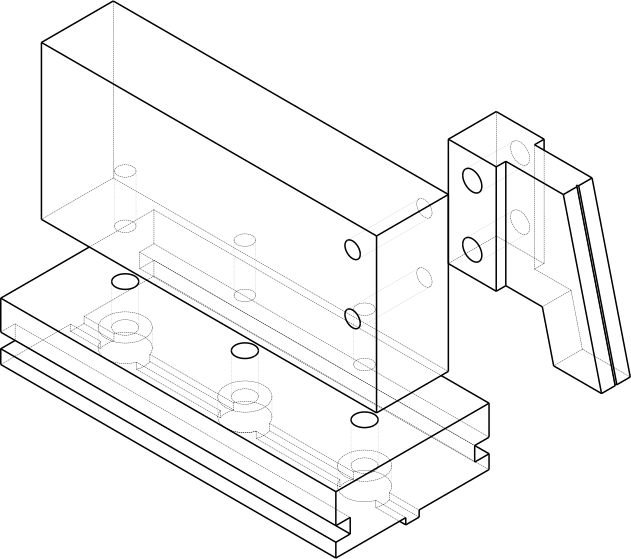
\includegraphics[height=8cm]{figures/supporto_completo.pdf}
	\caption{Exploded-view drawing of the fiber holder design.
	The holder is composed by three pieces.
	The tip is made of iron, in order to be used together with small magnets.}
	\label{fig:holders}
\end{figure}

Since the \acp{PIC} developed for IRIS support \acs{TE} modes only, after the positions of the optical fibers have been optimized, the coupled signal is maximized by the use of a polarizer.
The polarizer, placed between the fiber coupler and the sample, is a device composed by a long optical fiber.
Such fiber is coiled in three separate loops which have the effect of a half-wave plate, one quarter-wave plate, and another half-wave plate respectively.
Each coil can be manipulated, in a similar manner to the bulky quater-/half-wave plates, to change the output (linear) polarization of the light.
%The position of the polarization stage before of after the \ac{OSA} junction is not relevant as the \ac{OSA} is polarization independent.

In order to further reduce the impact of noise on measures, I also boxed the three linear stages with a rigid enclosure.
This decreased the noise, due to the movement of the fiber tips in air by at least one order of magnitude.

For the initial characterization, I studied the response of each output at input signals with low optical power and in the working range of the grating couplers, to identify the position of the resonances and their shape.
%As shown in \autoref{fig:M3sweep}, the through channel $th$ follows the shape of the grating coupler response, which is centered around \SI{1540}{\um} and slowly drops with the growing relative distance from that wavelength.
\autoref{fig:M3sweep} shows the normalized transmission of the eight drop channel ($dr_1$ to $dr_8$ ) and the through channel ($th$).
The first drop channel ($dr_1$) has the expected lorentzian shape, with a free spectral range of $FSR=\SI{19.2+-.1}{\nm}$, while the shapes of all the other drop channels are highly distorted because of the light collected by $dr_1$.
%On the other hand, all the other drop channels show a transmission that is perturbed by the light collected in the first channel.

\begin{figure}[htbp]
	\centering
%	\input{tikz/M1.tex}
%	\input{tikz/M2.tex}
	\tikzsetexternalprefix{tikz/}	% set subfolder
\tikzsetnextfilename{M3}

\begin{tikzpicture}[baseline]

	\definecolor{color1}{rgb}{0.12156862745098,0.466666666666667,0.705882352941177}
	\definecolor{color2}{rgb}{1,0.498039215686275,0.0549019607843137}
	\definecolor{color3}{rgb}{0.172549019607843,0.627450980392157,0.172549019607843}
	\definecolor{color4}{rgb}{0.83921568627451,0.152941176470588,0.156862745098039}
	\definecolor{color5}{rgb}{0.580392156862745,0.403921568627451,0.741176470588235}
	\definecolor{color6}{rgb}{0.549019607843137,0.337254901960784,0.294117647058824}
	\definecolor{color7}{rgb}{0.890196078431372,0.466666666666667,0.76078431372549}
	\definecolor{color8}{rgb}{0.45,0.45,0.45}
	\definecolor{color9}{rgb}{0.25,0.25,0.99}
	
	\begin{axis}[
			title={Output Power},
			xlabel={Wavelength [\si{\nm}]},
			ylabel={Transmission},
%			tick align=outside,
%			tick pos=left,
			width=\textwidth*0.75,%
			height=207pt,
			legend pos = outer north east,
			cycle list name=color list,
			/pgf/number format/1000 sep=,
			xtick distance=3,
			minor x tick num=2,
			minor y tick num=1,
		]
    
		\addlegendentry{\hspace{-.6cm}output}
		\addlegendimage{empty legend};
		\addlegendentry{\hspace{-.6cm}channel}
		\addlegendimage{empty legend};
		
%	  \pgfplotstableread[col sep=tab]{tikz/M1.csv}\tableM1
	  
    \pgfplotsinvokeforeach{1,2,...,8}{
        \addplot [semithick, color#1] table [x index=0, y index=#1] {tikz/m3.csv};
        \addlegendentryexpanded{ $dr_#1$ }
    }
		\addplot [semithick, color9] table [x index=0,y index=9] {tikz/m3.csv};
    \addlegendentry{ $th$ }
    
	\end{axis}
\end{tikzpicture}
	\caption{
		Transmission spectra of the drop channels ($dr_1$ to $dr_8$) and through channel $th$, average over five consecutive measures.
		The $dr_1$ channel shows the expected shape, whereas the other drop channels are clearly disturbed by the first one.
		The through channel shows a shape similar to the expected one, but it is actually the results of all the drop channels.
	}
	\label{fig:M3sweep}
\end{figure}

Another interesting fact is that the peak transmission of $dr_1$ channel is higher than the maximum transmission of $th$.
This is due to two factors: primarily the coupling maximization process with the linear stages has a repeatability error of about \SI{10}{\percent}, secondarily the $th$ channel is a longer structure and hence its losses are expected to be higher than the 'shorter` $dr_1$ channel.

Since $dr_1$ is the only channel with an unperturbed transmission, I focused my attention on its response only.
Specifically, I studied the resonance near \SI{1551.9}{\um}: % because it was the one with the highest transmitted signal and hence provided a better \acs{SNR}.
\autoref{fig:M3_1550_resonance} shows such resonance and highlights its width to $FWHM=\SI{0.6+-0.05}{\nm}$.
The estimated quality factor is $Q=\num{2600+-200}$.

\begin{figure}[!hbtp]
	\centering
	\tikzsetexternalprefix{tikz/}	% set subfolder
\tikzsetnextfilename{M3resonance}

\begin{tikzpicture}[baseline]

	\definecolor{color1}{rgb}{0.12156862745098,0.466666666666667,0.705882352941177}
%	\definecolor{color2}{rgb}{1,0.498039215686275,0.0549019607843137}
%	\definecolor{color3}{rgb}{0.172549019607843,0.627450980392157,0.172549019607843}
%	\definecolor{color4}{rgb}{0.83921568627451,0.152941176470588,0.156862745098039}
%	\definecolor{color5}{rgb}{0.580392156862745,0.403921568627451,0.741176470588235}
%	\definecolor{color6}{rgb}{0.549019607843137,0.337254901960784,0.294117647058824}
%	\definecolor{color7}{rgb}{0.890196078431372,0.466666666666667,0.76078431372549}
%	\definecolor{color8}{rgb}{0.45,0.45,0.45}
%	\definecolor{color9}{rgb}{0.25,0.25,0.99}
	
	\begin{axis}[
			title={Output Power},
			xlabel={Wavelength [\si{\nm}]},
			ylabel={Output Power [\si{\uW}]},
			tick align=outside,
			tick pos=left,
			width=\textwidth*0.75,%
			height=207pt,
			legend pos = north east,
			cycle list name=color list,
			xmin=1547, xmax=1557,
			/pgf/number format/1000 sep=,
		]
    
		\addlegendentry{\hspace{-.6cm}output}
		\addlegendimage{empty legend};
		\addlegendentry{\hspace{-.6cm}channel}
		\addlegendimage{empty legend};
		
%	  \pgfplotstableread[col sep=tab]{tikz/M1.csv}\tableM1
	  
		\addplot [semithick, color1] table [x index=0, y index=1] {tikz/M3.csv};
		\addlegendentryexpanded{ $dr_1$ }
		
		\draw [<-] (1552.55, 0.019) -- (1553.05, 0.019) node [right] {\scriptsize $FWHM$}; %0.5665693/2 = 0.283
		\draw [<-] (1551.80, 0.019) -- (1551.30, 0.019) {};
    
	\end{axis}
\end{tikzpicture}
	\caption{
		Resonance at \SI{1551.9}{\nm}, transmission to the drop port $dr_1$, average over five consecutive measures.
%		This spectrum is the only one unperturbed by the other transmission spectra.
%		The FWHM and the resonance wavelength are clearly visible in the figure.
	}
	\label{fig:M3_1550_resonance}
\end{figure}

\section{Characterization of the Activation Function}
\label{sec:Characterization_of_the_Activation_Function}
To characterize the nonlinear response of the microring resonator the setup used for the initial measures has been modified.
To induce the thermal bistability effect in the microring the signal of the TUNICS has been amplified using an \ac{EYDFA}.
%Even more so with the addition of the optical amplifier, the role of the circulator placed between the sources and the rest of the devices is of fundamental importance.
In this configuration, the role of the circulator placed between the sources and the rest of the devices acquires even more importance, as back-reflected signals that enter optical amplifier in the wrong direction can cause serious damage to the equipment.

In addition to the amplifying stage, a remotely controlled \ac{VOA} was added between the polarizer and the sample, to quantitatively characterize the nonlinear response of the microring. %the response of the microring resonator to signals of fixed wavelength but different optical power.
The \ac{VOA} employed is controlled by a voltage signal in the range \SIrange{0}{5}{\V}: it provides full transparency for \SI{0}{\V} and full attenuation for \SI{5}{\V} and, in between, the attenuator behaves similarly to a sigmoid function, shown in \autoref{fig:VOA}.
This curve has been identified with its closest analytical polynomial, to obtain an inverse formula that links transparency values in the range $[0,1]$ to the respective correct voltage value.

\begin{figure}[htbp]
	\centering
	\tikzsetexternalprefix{tikz/}	% set subfolder
\tikzsetnextfilename{VOA}

\begin{tikzpicture}[	baseline ]
	
	\begin{axis}[
			title={VOA Calibration},
			xlabel={Control Signal [\si{\V}]},
			ylabel={VOA Transparency},
			width=\textwidth*0.75,%
			height=207pt,
			legend pos = outer north east,
		]
		
    \addplot [mark=+] table [x index=0, y expr=\thisrowno{1}/1.519545] {tikz/VOA_calibration.csv};
    
	\end{axis}
	
\end{tikzpicture}
	\caption{Typical calibration curve of the attenuation curve of the VOA.
		The data has been fitted with a spline to implement online control over the attenuation value.
	}
	\label{fig:VOA}
\end{figure}%1.519545

This setup successfully induces the nonlinear response in the microring for detunings up to values comparable to half $FWHM$.
However, instabilities of the source and the amplification stages in the optical power and in the wavelength of the signal increase the uncertainty on the measures.
Specifically, the system shows a drift in optical power immediately after the source and amplification stages are switched on and random noise of the order of \SI{0.1}{\percent}.
Moreover, the wavelength of the light generated shows a slow drift toward shorter wavelengths, which becomes important for long measurements.
The typical wavelength stability of the source is rated at \SI[per-mode=symbol]{+-3}{\pico\meter\per\hour} (from instrument datasheet).

The first corrective measure is obtained by allowing the system to thermalize.
The most critical instrument is the \ac{EYDFA}, which might take up to half an hour to reach a steady state.
This step reduces the slow drift in the output power of the source, but does not suppress the instantaneous noise in power and wavelength of the signal.

In order to provide a correction for the instantaneous noise, a small part of the signal is collected from the main path, before the VOA, via a fiber coupler (99\%:1\%) and it is the equally distributed via a second fiber coupler (50\%:50\%) to the OSA and to a second infrared \ac{PD} (PD-B).
The completed setup is shown in \autoref{fig:pump_setup}.

\begin{figure}[hbtp]
	\centering
	\tikzsetnextfilename{pump_setup}
% Define size/space
\def\loopsize{.8cm}
\def\loopoffset{0.2cm}
% Define the loops
\def\myloops#1#2{
\begin{scope}[shift={#1}, scale=#2]
        % Draw the baseline
    \draw (-\loopoffset,0) -- (\loopoffset,0);
        % Draw the loops
    \draw (-\loopoffset,0)	node [draw, thick, circle, anchor=south, minimum size=\loopsize] (id) {};
    \draw (0,0) 						node [draw, thick, circle, anchor=south, minimum size=\loopsize] (id) {};
    \draw (\loopoffset,0) 	node [draw, thick, circle, anchor=south, minimum size=\loopsize] (id) {};
\end{scope}
}

\begin{tikzpicture}
	[
	source/.style ={
		draw, rectangle, inner sep=6pt, anchor=west
		},
	VOA/.style ={
		draw, circle, inner sep=2pt, fill=white, anchor=west
		},
	sample/.style={
		draw, chamfered rectangle, chamfered rectangle=8pt, anchor=west
		},
	coupler/.style={
		draw, rounded rectangle, rounded rectangle right arc=none, anchor=west, inner sep=2pt
		},
	thick,
	] %radius=5, inner sep=0pt,	minimum size=3mm}
	
	\draw (0,0) node [source, align=center] (tunics)
									{\small TUNICS\\\tiny + \\\small EYDFA}
					node [above] at (tunics.north) {source}
					node [below] at (tunics.south) {amplified}
				(tunics.east)
%				++(0.6, 0) node [source] (eydfa) {EYDFA}
%					node [above] at (eydfa.north) {amplifier}
%				(eydfa.east)
				++(0.6, 0) node [VOA] (circ) {$\scriptstyle\circlearrowright$}
%					node [above] at (circ.north) {circ}
			  (circ.east)
				++(0.6, 0) node [coupler] (couplerA) {\tiny(a)}
					node [above] at (couplerA.north east) {\tiny .5}
					node [below] at (couplerA.south east) {\tiny .5}
			   +(1.0,-1.2) node [source] (osa) {OSA}
					node [below] at (osa.south) {detector}
				(couplerA.east)
				++(1.2, 0) node (polarizer) {}
				++(1.2, 0) node [coupler] (couplerB) {\tiny(b)}
					node [above] at (couplerB.north east) {\tiny .9}
					node [below] at (couplerB.south east) {\tiny .1}
				(couplerB.east)
				++(1.0, 0) node [VOA] (voa) {$\scriptstyle\nearrow$}
					node [above] at (voa.north) {voa}
			   +(0.0,-1.2) node [source] (detectorB) {Ge B}
					node [below] at (detectorB.south) {detector}
			  (voa.east)
				++(0.6, 0) node [sample] (sample) {sample}
				(sample.east)
				++(0.6, 0) node [source] (detectorA) {Ge A}
					node [above] at (detectorA.north) {detector};
	
	\myloops{(polarizer)}{1}
	\node [below] at (polarizer) {polarizer};

	\draw (tunics) -- ++(circ) node [pos=.85, above] {\tiny (1)}
				(circ) -- (couplerA) node [pos=.15, above] {\tiny (2)}
				(circ) to [out=225, in=90] ++(-0.4,-0.6) node [circle, inner sep=1pt, black, fill=black] {}
																								node [below] {\tiny (3)}
				(circ) to [out=315, in=90] ++(+0.4,-0.6) node [circle, inner sep=1pt, black, fill=black] {}
																								node [below] {\tiny (4)}
				(couplerA.20) to [out=0, in=180] (polarizer)
				(couplerA.-20) to [out=0, in=180] (osa)
				(polarizer) to (couplerB)
				(couplerB.20) to [out=0, in=180] (voa)
				(couplerB.-20) to [out=0, in=180] (detectorB)
				(voa) -- (sample)
				(sample) -- (detectorA)
				;

\end{tikzpicture}
	\caption{Scheme of the setup used to obtain characterization of the thermal bistability in the microring resonator.
		The source (TUNICS) is amplified by an \acs{EYDFA} and is followed by the circulator and by the polarizer.
		Then a small part of the signal is collected by a fiber coupler (99\%:1\%) and it is equally distributed between the OSA and an additional infrared \ac{PD} (PD-B).
		The signal in the main path passes through a \acf{VOA}, then it is injected into the sample, and finally extracted to be read by the first \ac{PD} (PD-A).
		}
	\label{fig:pump_setup}
\end{figure}

In this configuration, PD-B measures the instantaneous power in input at the VOA and, together with the value of transparency selected on the VOA, provides control over effective power coupled into the \ac{PIC} and correction over the noise in the power of the source.
The sampling rate of PD-B is the same of PD-A and is limited by the acquisition board (\SI{1}{\kHz}).

On the other hand, the \ac{OSA} provides a check over the wavelength of the source, but no correction can be implemented.
Moreover, the measures obtained by means of the \ac{OSA}, due to intrinsic limitations of the instrument and to the high complexity of the measure itself, have a much lower sampling rate in comparison to the measures given by the \acp{PD}.

Since this setup has been employed to measure several times the hysteresis cycle, for the same input wavelength, the measurement could run for several minutes consecutively.
In order to collect a significant number of points, without important drifts in the signal wavelength, the sampling time had to be reduced as much as possible.
For this reason, the \ac{OSA} has been employed as a check on the signal wavelength, before and after each measure of the hysteresis loops.

%On the other hand, the second infrared detector was inserted in the measuring loops such that it collected data for each sampled point.
To summarize, the data collected is composed by the optical power measured before the \ac{VOA}, by the transparency of the \ac{VOA}, and by the optical power measured at the output.
This three-point measurement allows more robustness against power fluctuations.

%Other than the addition discussed so far, the system setup is very similar to the one used before.
%The coupling system and alignment process of the sample are the same described above in \autoref{ssec:initial_characterization}.

\subsection{Bistability wavelength dependence}
\label{ssec:bistability_wavelength_dependence}
The first feature studied is the dependence of the overall shape of the bistability hysteresis loop on wavelength detuning.
As seen in \autoref{ssec:Simulations}, the form of the bistability changes with the detuning from the resonant wavelength.
This behavior is also observed in the transmission spectra experimentally measured, as shown in \autoref{fig:bistability_shape}.

\begin{figure}[hbtp]
	\centering
	\tikzsetexternalprefix{tikz/}	% set subfolder
\tikzsetnextfilename{shapes}

\newcommand{\plotshape}[1]{
    \pgfplotstableread[col sep=tab, header=true]{#1}{\table}
    \pgfplotstablegetcolsof{#1}
    \pgfmathtruncatemacro\numberofcols{\pgfplotsretval - 1}
    \pgfplotsinvokeforeach{1,...,\numberofcols}{
        \pgfplotstablegetcolumnnamebyindex{##1}\of{\table}\to{\colname}
        \addplot [semithick, color##1, mark=*, mark size=1]%
        		table [x index= 0, y index=##1] {#1};
        \addlegendentryexpanded{ \colname }
    }
}

\begin{tikzpicture}[baseline]

	\definecolor{color1}{rgb}{0.12156862745098,0.466666666666667,0.705882352941177}
	\definecolor{color2}{rgb}{1,0.498039215686275,0.0549019607843137}
	\definecolor{color3}{rgb}{0.172549019607843,0.627450980392157,0.172549019607843}
	\definecolor{color4}{rgb}{0.83921568627451,0.152941176470588,0.156862745098039}
	\definecolor{color5}{rgb}{0.580392156862745,0.403921568627451,0.741176470588235}
	\definecolor{color6}{rgb}{0.549019607843137,0.337254901960784,0.294117647058824}
	\definecolor{color7}{rgb}{0.890196078431372,0.466666666666667,0.76078431372549}
	\definecolor{color8}{rgb}{0.45,0.45,0.45}
	\definecolor{color9}{rgb}{0.25,0.25,0.99}
	\definecolor{color10}{rgb}{0.0,0.0,0.0}
	\definecolor{color11}{rgb}{0.12156862745098,0.466666666666667,0.705882352941177}
	\definecolor{color12}{rgb}{1,0.498039215686275,0.0549019607843137}
	\definecolor{color13}{rgb}{0.172549019607843,0.627450980392157,0.172549019607843}
	\definecolor{color14}{rgb}{0.83921568627451,0.152941176470588,0.156862745098039}
	\definecolor{color15}{rgb}{0.580392156862745,0.403921568627451,0.741176470588235}
	\definecolor{color16}{rgb}{0.549019607843137,0.337254901960784,0.294117647058824}
	\definecolor{color17}{rgb}{0.890196078431372,0.466666666666667,0.76078431372549}
	\definecolor{color18}{rgb}{0.45,0.45,0.45}
	\definecolor{color19}{rgb}{0.25,0.25,0.99}
	
	\begin{axis}[
			title={Internal Power},
			xlabel={Pump Power [\si{mW}]},
			ylabel={Internal Power [arb.units]},
%			tick align=outside,
			tick pos=left,
			width=\textwidth*0.75,%
			height=207pt,
			legend pos = outer north east,
			cycle list name=color list,
			forget plot style={opacity=0.4},
		]
		\addlegendentry{\hspace{-.6cm}$\Delta\lambda$ in \si{\pm}}
		\addlegendimage{empty legend};
		
		\plotshape{tikz/shapes.csv}
		
	\end{axis}
\end{tikzpicture}
	\caption{Many bistability loops at different wavelengths.
		The loops that are closer to the microring resonance have smaller bistability regions or they have not one at all.
		Loops that are farther from the resonance have larger bistability regions.}
	\label{fig:bistability_shape}
\end{figure}

As expected, the region of bistability disappears into a sigmoid for small detunings, while becomes larger for increased detunings.
The range of wavelengths with which the sample has been probed is upper limited due to the growing pump power required to activate the bistability.

Even though the behavior observed experimentally is similar to the one obtained with the simulations, there are some differences:
first of all, in the experiments the transmission for high input power saturates at the same value for different detunings.
Moreover, in the experiment all wavelengths shows a peak and a decrease in transmission from a certain level of input power.
On the contrary, in the simulations the output power does not saturate and shows different transmission efficiency for each detuning (see \autoref{fig:sim_bist_cycle}).

Several are the factors that might produce these discrepancies between the experiments and the simulations.
First of all, the setup and especially the sample are composed by many different structures.
Each of them has its unique response to high values of optical power.
Secondly, the parameters employed in the simulation are an estimate of the actual parameters that define the microring resonator and its coupling with the waveguides.
Lastly, the theoretical model implemented in the numerical calculations is an approximation of the physical phenomena that occur in the system.

\subsubsection{Bistability region edges}
\label{sssec:bistability_region_edges}
In order to precisely characterize the abrupt jumps on the edges of the bistability region, the stability of the system is crucial.
Hence I implemented a specific series of measurements, which samples only the nearest part of the edge: the amount of points sampled is smaller, however the complete measurement is faster and the sampling near the bistability edges is more dense.

The first step of each measurement is setting the source wavelength at a specific value, which is measured by the \ac{OSA}.
Then the serial measurements begins: for ascending loops, at the beginning \ac{VOA} is initialized at full attenuation and then is used to sample the edge with small increasing steps.
For descending loops, the \ac{VOA} is initialized at full transparency and the steps are decreasing instead.
After the predefined number of loops is completed, the wavelength of the source is measured with the \ac{OSA} again.
%These loops repeatedly initialized the system with the \ac{VOA} at full absorption and then characterized the jump by sampling from few points below to few points above the bistability step.
%Similarly, the other \textit{inverse} bistability step was characterized by analogous loops in which the system was initialized with the VOA at full transparency instead.

The data collected included twenty loops for each detuning, which are five almost equally spaced in a wavelength range from \SIrange{1552.2}{1552.3}{\nm}.
Each set of data has been analyzed to find the abrupt jumps from a state to the other.
A simple study of the discrete derivative was employed to achieve that.
The same procedure has been applied both to the rising as well as to the descending loops.
The results are five data points for the first kind of loops and just as much for the descending one, as shown in \autoref{fig:bistability_jumps}.
The wavelength of each loop is measured by checks with the \acs{OSA} before the start and after the completion of each loop.

\begin{figure}[!hbtp]
	\centering
	\tikzsetexternalprefix{tikz/}	% set subfolder
\tikzsetnextfilename{jumps}

\begin{tikzpicture}[baseline]

%	\definecolor{color1}{rgb}{0.12156862745098,0.466666666666667,0.705882352941177}
%	\definecolor{color2}{rgb}{1,0.498039215686275,0.0549019607843137}
%	\definecolor{color3}{rgb}{0.172549019607843,0.627450980392157,0.172549019607843}
%	\definecolor{color4}{rgb}{0.83921568627451,0.152941176470588,0.156862745098039}
%	\definecolor{color5}{rgb}{0.580392156862745,0.403921568627451,0.741176470588235}
%	\definecolor{color6}{rgb}{0.549019607843137,0.337254901960784,0.294117647058824}
%	\definecolor{color7}{rgb}{0.890196078431372,0.466666666666667,0.76078431372549}
%	\definecolor{color8}{rgb}{0.45,0.45,0.45}
%	\definecolor{color9}{rgb}{0.25,0.25,0.99}
\pgfplotsset{myerr/.append style={only marks, mark size=1.5pt, error bars/.cd, y dir=both, y explicit, x dir=both, x explicit} }

\pgfplotsset{
  /pgfplots/error bar legend/.style={
    legend image code/.code={
			\draw [|-|] (0.15cm, 0cm) -- (0.45cm, 0cm);
			\draw [|-|] (0.3cm, -0.15cm) -- (0.3cm,0.15cm);
%			\draw [radius=1.5pt] circle (0,0);
			\draw[mark repeat=2,mark phase=2,##1]
			plot coordinates {(0cm,-0.2cm) (0.3cm,0cm) (0.6cm,0.2cm)};
    }
  }
}
	
	\newcommand{\Central}{1552}
	
	\begin{axis}[
			title={Bistability region power limits},
			xlabel={Wavelength Detuning [\si{\nm}]},
			ylabel={Output Power [\si{\uW}]},
			scaled x ticks = manual:{$+\SI{\Central}{\nm}$}{ \pgfmathparse{#1-\Central }},
			tick align=outside,
			tick pos=left,
			width=\textwidth*0.75,
			height=207pt,
			legend pos = north west,
			error bar legend,
		]
    
		\newcommand{\f}{0.6};
    
%		\addlegendentry{\hspace{-.6cm}output}
%		\addlegendimage{empty legend};

		\addplot [	red,
							myerr,
			] table [x=xmin,y=ymin, x error expr=\thisrow{xerror}/\f, y error expr=\f*\thisrow{yminerr}]
				{tikz/jumps.csv};
    \addlegendentry{lower limit};
    
		\addplot [	blue,
							myerr
			] table [x=xmax,y=ymax, x error expr=\thisrow{xerror}/\f, y error expr=\f*\thisrow{ymaxerr}]
				{tikz/jumps.csv};
    \addlegendentry{upper limit};
    
	\end{axis}
\end{tikzpicture}
	\caption{Wavelength dependence of the bistability region edges.
		Upper limits are shown as blue dots, while lower limits are shown as red dots.
		The wavelength is estimated by checks in betweens consecutive measures obtained with the \acs{OSA}.
		Its uncertainty is assumed to be \SI{5}{\pm} (TUNICS Wavelength Setting Repeatability) for all the points.
		The power uncertainty is given by the statistic of the data collected. % with the loop in power.
	}
	\label{fig:bistability_jumps}
\end{figure}

%The error on each point has been evaluated as follows.
The uncertainty on the wavelength position is assumed to be the \SI{5}{\pm} for all the points, which is the wavelength setting repeatability of the TUNICS.
The uncertainty on the power is evaluated from the statistic of all the loops measured at the same wavelength.
Hence it is defined as the RMS error of twenty data points for each wavelength.

It is interesting to observe that the experimental data, much like the simulations, show a steeper dependence on wavelength for the upper limits that for the lower limits.
Nevertheless, both quantities seem to increase with wavelength more distant from the resonance.
Moreover, the position of the edges of the bistability region seem to be precisely defined by the parameters of the system.

\section{Test of a Trained ANN}
\label{sec:Test_of_a_Trained ANN}
The first step I made to test the nonlinear response of a microring resonator as a neural network activation function was to exploit the fitted bistability curve of \autoref{eq:fit} and implement it as activation function of the model defined in \autoref{ssec:Simulated_ANN_operation}.

\subsection{Optical bistability as nonlinear activation function}
\label{ssec:Optical_bistability_as_nonlinear_activation_function}
Having obtained a description of the optical bistability of the response of a microring resonator in a wide range of wavelengths, I implemented the shape of such response in a simulated artificial neural network.
Hence, I chose a representative set of data:
%from the group, such that it was neither the most distant nor the closest to the resonance.
%This was made to avoid unexpected ``border effects''.
specifically, the data belongs to the increasing half of the bistability loop for input light at \SI{1552.300}{\nm} \ref{}.

\begin{figure}[htbp]
	\centering
	\tikzsetexternalprefix{tikz/}	% set subfolder
\tikzsetnextfilename{fit+residuals}

%['689.652', '0.434', '1.310', '-0.975', '-0.518', '0.403', '0.502']

\begin{tikzpicture}
	\begin{axis}[
			title={Nonlinear activation function fit},
			width=0.75\textwidth,
			height=207pt,
			scale only axis,
			name=main plot,
			xticklabels=\empty,
			domain=0:1,
			ylabel={Output signal},
			legend pos=south east,
	    clip mode=individual,			
		]

	\addplot [blue, thick, mark=*, mark size=1.2, mark options={green!70!blue}]
		table [x index=0, y index=1] {tikz/activation.csv};
		
	\addplot [red, thick, samples=501]
		{	+ 0.434 / (1 + exp(-689.652*(x-0.403) ))
			+ 1.310*max(x,0)
			- 0.975*max(x-0.403,0)
			- 0.518*max(x-0.502,0)
			}; % {b*sigmoid(a*(arg-x0))+c*relu(arg)+d*relu(arg-x0)+g*relu(arg-x1)};
	
	\addlegendentry{data points};
	\addlegendentry{fit};
	
	\end{axis}
	
	\begin{axis}[
			at={(main plot.below south west)},
			yshift=.2cm,
			xlabel={Input signal},
			ylabel={Residuals},
			anchor=north west,
	width=0.75\textwidth,
			scale only axis,
			height=1.6cm,
			domain=0:1,
			ymin=-0.12, ymax=+0.12,
			ytick={-0.1,0,0.1},
	    clip mode=individual,
		]
	
	\addplot [thick, blue, mark=*, mark size=1.2, mark options={green!70!blue, solid}]
		table [x index=0, y index=2] {tikz/activation.csv};
		
	\addplot [thick, red] table [x index=0, y index=1] {tikz/residuals.csv};

	\end{axis}
\end{tikzpicture}
	\caption{Curve fitting and residuals on a set of data.
	The nonlinear curve is the increasing half of a bistability loop.
	The fit is quite close to the original values, except near the jump.}
	\label{fig:fit+residuals}
\end{figure}

The curve employed to fit the data is a combination of function that are already implemented in PyTorch library.
This allows a simple implementation in the simulations.
Specifically the function is composed by \textit{Logistic} and \textit{ReLU} function
\begin{equation}
	f_{fit} \defeq b~f_{Logistic}\left[a(x-x_0)\right] + c~f_{ReLU}\left[x\right]+d~f_{ReLU}\left[x-x_0\right]+e~f_{ReLU}\left[x-x_1\right],
	\label{eq:fit}
\end{equation}
where the parameters $a$, $b$, $c$, $d$, $e$, $x_0$, and $x_1$ are fixed by the fit.

As shown in \autoref{fig:fit+residuals}, the curve fit on the chosen dataset is very close to the original data points.
This is true all over the range of powers, except near the bistability edge, where the maximum difference occurs.

\subsection{Optical bistability vs ReLU and Logistic}
\label{ssec:OBvsReLUvsSIGM}
HO PROVATO DIVERSE GEOMETRIE e DIVERSE LOSS FUNCTIONS\\
COME ADATTARE I PESI VIRTUALI A QUELLI FISICI? rappresentazione a bassa precisione?


\begin{figure}[htbp]
	\centering
	\input{tikz/Train_evolution_OB.tex}
	\caption{Evolution of the loss criterion (solid lines) throughout the epochs.
		Points represent the values of the loss criterion on the validation dataset, carried out repeatedly during the training.
	}
	\label{fig:fit_learning}
\end{figure}

\autoref{fig:fit_learning} shows the evolution of the loss and the validation of each model during the \num{2000} epochs of training.
From the evolution of the loss function we can see that every model has 

The percentage of correct answer of different models that implements the optical bistability activation function is given by \autoref{tab:ExpResults}.
The same shapes have been tested with $f_{ReLU}$ and $f_{Logistic}$ in \autoref{ssec:Simulated_ANN_operation}.

\begin{table}[htbp]
	\centering
	\begin{tabular}{c c c c r}
	\toprule
	activation	& no. hidden 	& no. nodes	& other			& Percent\\
	function		& layers 			& per layer	& parameters	& correct\\
	\midrule
	$f_{fit}$ 			& 2 & 11 & - & \SI{66}{\percent}\\
	$f_{fit}$ 			& 2 & 22 & - & \SI{55}{\percent}\\
	$f_{fit}$ 			& 3 & 11 & - & \SI{44}{\percent}\\
	$f_{fit}$ 			& 3 & 22 & - & \SI{33}{\percent}\\
	\bottomrule
	\end{tabular}
	\caption{Results of the $f_{fit}$ function for several network topologies.
	}
	\label{tab:ExpResults}
\end{table}

As we can see the performance of the $f_{fit}$ function lies in the range of the $f_{ReLU}$, even if a bit lower.


% conclusive chapter ~ 5pg
\chapter*{Conclusion}
\markboth{CONCLUSION}{}
\addcontentsline{toc}{chapter}{Conclusions}

% total ~ 60pg

% Bibliography
%\cleardoublepage
\printbibliography[heading=bibintoc]%,title={References}]

% Aknowledgements
\chapter*{Aknowledgements}
\markboth{AKNOWLEDGEMENTS}{}
\addcontentsline{toc}{chapter}{Aknowledgements}

\end{document}